\documentclass[a4paper,UKenglish]{lipics-v2016}
\usepackage{microtype}
\usepackage{amssymb,amsmath}
\usepackage{graphics,graphicx,color}
\usepackage{enumerate,paralist,hyperref}
\usepackage{caption,subcaption,xspace}
\usepackage{todonotes} 
\usepackage{times,setspace} 

%%%% Title of contribution
% ==================================================================
\title{Characterizations of Optimal 2- and 3-planar Graphs}
\titlerunning{Characterizations of Optimal 2- and 3-planar Graphs}
\author[1]{Michael~A.~Bekos}
\author[1]{Michael~Kaufmann}
\author[2]{Chrysanthi~N.~Raftopoulou}
% ==================================================================
\affil[1]{
Wilhelm-Schickhard-Institut f\"ur Informatik, Universit\"at T\"ubingen, Germany\\
\texttt{\{bekos,mk\}@informatik.uni-tuebingen.de}}
\affil[2]{
School of Applied Mathematical \& Physical Sciences, NTUA, Greece\\
\texttt{crisraft@mail.ntua.gr}}
% ==================================================================

% ==================================================================
\authorrunning{Michael~A.~Bekos, Michael~Kaufmann, Chrysanthi~N.~Raftopoulou}
% ==================================================================

\Copyright{Michael~A.~Bekos, Michael~Kaufmann, Chrysanthi~N.~Raftopoulou}
\subjclass{G.2.2 Graph Theory}% mandatory: Please choose ACM 1998 classifications from http://www.acm.org/about/class/ccs98-html . E.g., cite as "F.1.1 Models of Computation".
\keywords{$k$-planar graphs, characterization, graph drawing}%

%%%%%%%%%%%%%%%%%%%%%%%%%%%%%%%%%%%%%%%%%%%%%%%%%%%%%%%%%
%Editor-only macros (do not touch as author)
\EventEditors{Boris Aronov, Matthew Katz}
\EventNoEds{1}
\EventLongTitle{33rd International Symposium on Computational Geometry}
\EventShortTitle{SoCG 2017}
\EventAcronym{SoCG}
\EventYear{2017}
\EventDate{July 4-7, 2017}
\EventLocation{Brisbane, Australia}
\EventLogo{}
\SeriesVolume{}
\ArticleNo{X} % Your paper number goes here! (not your EasyChair submission number)
%%%%%%%%%%%%%%%%%%%%%%%%%%%%%%%%%%%%%%%%%%%%%%%%%%%%%%%%%

\newtheorem{property}{Property}

\newcommand{\pe}{potential edge\xspace}
\newcommand{\pes}{potential edges\xspace}
\newcommand{\pp}{potential empty cycle\xspace}
\newcommand{\pr}{potential region\xspace}
\newcommand{\pb}{potential boundary\xspace}

\newcommand{\parallelsum}{\mathbin{/\mkern-4mu/}}
\newcommand{\ppp}[2]{\angle [#1,#2]}
\newcommand{\ppc}[2]{\parallelsum [#1,#2]}

\begin{document}
\maketitle

% ============================================================================
\begin{abstract}
$k$-planarity is a concept that extends the class of planar graphs by allowing graphs that can be drawn with at most $k$ crossings on each edge. While for $1$-planar graphs, the \emph{optimal} graphs, i.e., those with the maximum number of edges, have been completely characterized, this was not the case for $k \geq 2$. For such cases, in particular for $k=2,3$ and $4$, upper bounds on the number of edges have been developed for the case of simple graphs by Pach and Toth, Pach et al.\ and Ackerman. Since then the bounds are known to be achieved by graphs with a very regular structure; the set of uncrossed edges form pentagonal or hexagonal faces respectively, which then are completely by $5$ more edges in the pentagons for the $2$-planar case, and by $8$ more edges in the hexagons for the $3$-planar case. Unfortunately, non-homotopic parallel edges have to be allowed. Previously, we have shown that the known bounds for the simple graphs hold also for the case of non-simple graphs with non-homotopic parallel edges and loops. In this paper, we prove that only those graphs achieve the bound of $5n-10$ for $2$-planar and the $5.5n -11$ bound for $3$-planar graph and provide a complete characterization of optimal non-simple $2$- and $3$-planar graphs.
\end{abstract}
% ============================================================================

% ============================================================================
\section{Introduction}
\label{sec:introduction}
% ============================================================================

The gradually improvement of the well-known lemma of crossing numbers \cite{ACNS82,Lei83}, but also recent interest in graphs beyond planarity gave rise to multiple extensions of planar graphs allowing edge crossing in some restricted local configurations. The most prominent is the concept of $k$-planarity; here each edge can be crossed at mot $k$ times. Earlier work mainly considered the case $k=1$, i.e., $1$-planar graphs. We mention here the coloring problem of 1-planar graphs by Ringel~\cite{Ringel65} and the first density bounds by Bodendiek, Schumacher and Wagner~\cite{BSW84}. Later on, Suzuki \cite{DBLP:journals/siamdm/Suzuki10} gave simple rules how to generate maximal $1$-planar graphs. Other works considered maximal 1-planar graphs~\cite {DBLP:conf/gd/BrandenburgEGGHR12} and recognition of $1$-planar graphs~\cite{DBLP:journals/corr/Brandenburg16a}. But also subclasses have been considered like \emph{IC-planar graphs}, where for each vertex, only one incident edge can be crossed \cite{DBLP:conf/gd/BrandenburgDEKL15}, and several others on outer-1-planarity where all the vertices have to be adjacent to the outer face as being required in the corresponding model of outer-planarity~\cite{DBLP:journals/algorithmica/HongEKLSS15,DBLP:journals/jgaa/GiacomoLM15,DBLP:journals/algorithmica/AuerBBGHNR16}.

For larger $k \geq 2$, the paper of Pach and Toth~\cite{PachT97} provided significant progress, as it gives techniques for upper bounds on the edge density for simple $k$-planar graphs, which then lead to upper bounds of $5n -10$ for $2$-planar, $6n -12$ for $3$-planar and $7n-13$ for $4$-planar graphs. For larger $k$, the authors provide a bound of $4.1 \sqrt k n$. While the bound for $2$-planar graphs is tight, the other bounds have been improved to $5.5n - 11$ \cite{PachRTT06} and $6n-12$ \cite{DBLP:journals/corr/Ackerman15} for simple $3$- and $4$-planar graphs, respectively. In our companion paper~\cite{BKR16}, we generalize the result and the bound of Pach et al.~\cite{PachRTT06} to non-simple graphs, where non-homotopic parallel edges as well as non-homotopic selfloops are allowed.

In this paper, we now completely characterize optimal non-simple $2$-planar and $3$-planar graphs, i.e., those that achieve the bound of $5n-10$ and $5.5n-11$ on the number of edges, respectively. In particular, we prove that the commonly known $2$-planar graphs that achieve the upper bound of $5n-10$ are the only optimal $2$-planar graphs. Such graphs consist of a crossing-free subgraph where all faces have size $5$, which then are enhanced by $5$ more edges forming a $K_5$'s together with the boundary edges of the face (Section~\ref{sec:2planar}). For $3$-planar graphs, we can show correspondingly that optimal $3$-planar graphs have a similar simple structure (Section~\ref{sec:3planar}).

Related to this work are also other extensions of planarity, like fan-planarity \cite{KU14,DBLP:conf/gd/BekosCGHK14,DBLP:journals/tcs/BinucciGDMPST15,DBLP:conf/gd/BinucciCDGKKMT15}, quasi-planarity \cite{AAPPS97,DBLP:journals/cj/GiacomoDLMW15}, k-quasi-planarity~\cite{DBLP:conf/gd/Suk11,DBLP:journals/comgeo/SukW15}, RAC drawability~\cite{DBLP:journals/tcs/DidimoEL11,DBLP:journals/jgaa/ArgyriouBS12}, and fan-crossing-free planarity~\cite{DBLP:journals/algorithmica/CheongHKK15} 
as well as alternative geometric representations like bar-1 visibility~\cite{DBLP:conf/icaa/SultanaRRT14,DBLP:journals/jgaa/Evans0LMW14,DBLP:conf/walcom/BrandenburgEN16} and more in general bar-$k$ visibility~\cite{DBLP:journals/dm/GenesonKT14,DBLP:journals/corr/SawhneyW16}. Note that all aforemention classes of nearly-planar graphs have also linear number of edges (except for the classes of $k$-quasi planar and bar-$k$ visibile graphs, whose number of edges also depends on the parameter $k$). 


% ============================================================================
\section{Preliminaries}
\label{sec:preliminaries}
% ============================================================================

Let $G$ be a (not necessarily simple) \emph{topological graph}, that is, $G$ is a graph drawn on the plane, so that the vertices of $G$ are distinct points in the plane, its edges are Jordan courves joining the corresponding pairs of points, and:%
%
\begin{inparaenum}[(i)]
\item no edge passes through a vertex different from its endpoints, 
\item no edge crosses itself and 
\item no two edges meet tangentially.
\end{inparaenum}
Let $\Gamma(G)$ be such a drawing of $G$. The \emph{crossing graph} $\mathcal{X}(G)$ of $G$ has a vertex for each edge of~$G$, while two vertices of $\mathcal{X}(G)$ are connected by an edge if and only if the corresponding edges of $G$ cross in $\Gamma(G)$. A connected component of $\mathcal{X}(G)$ is called \emph{crossing component}. Observe that the set of crossing components of $\mathcal{X}(G)$ define a partition of the edges $G$. Given an edge $e$ of $G$ we denote by $\mathcal{X}(e)$ the crossing component of $\mathcal{X}(G)$ which contains $e$. 

An edge $e$ in $\Gamma(G)$ is called a \emph{topological edge} (or simply edge, if this is clear in the context). Edge $e$ is called \emph{true-planar}, if it is not crossed by any other edge in $\Gamma(G)$. The set of all true-planar edges of $\Gamma(G)$ forms the so-called \emph{true-planar skeleton} of $\Gamma(G)$, which we denote by $\Pi(G)$. Since $G$ is not necessarily simple, we will further assume that $\Gamma(G)$ contains neither \emph{homotopic parallel edges} nor \emph{homotopic self-loops}, that is, both the bounded and the unbounded regions defined by any self-loop or by any pair of parallel edges contain at least one vertex in their interiors. For a possitive integer $s$, a cycle of length $s$ is called \emph{true-planar $s$-cycle} if it consists of true-planar edges of $\Gamma(G)$. Note that if $e$ is a chord of a true-planar $s$-cycle that has no vertices in its interior, then all edges of $\mathcal{X}(e)$ are also chords of this $s$-cycle. Let $\mathcal{F}_s=\{v_1,v_2,\ldots,v_s\}$ be a facial $s$-cycle of $\Pi(G)$ with length $s \geq 3$.  The order of the vertices (and subsequently the order of the edges) of $\mathcal{F}_s$ is determined by a walk around the boundary of $\mathcal{F}_s$ in clockwise direction. Since $\mathcal{F}_s$ is not necessarily simple, a vertex (or an edge, respectively) may appear more than once in this order; see Figure~\ref{fig:non_simple_face}.

\begin{figure}[tb]
    \centering	
	\begin{minipage}[b]{.18\textwidth}
        \centering
        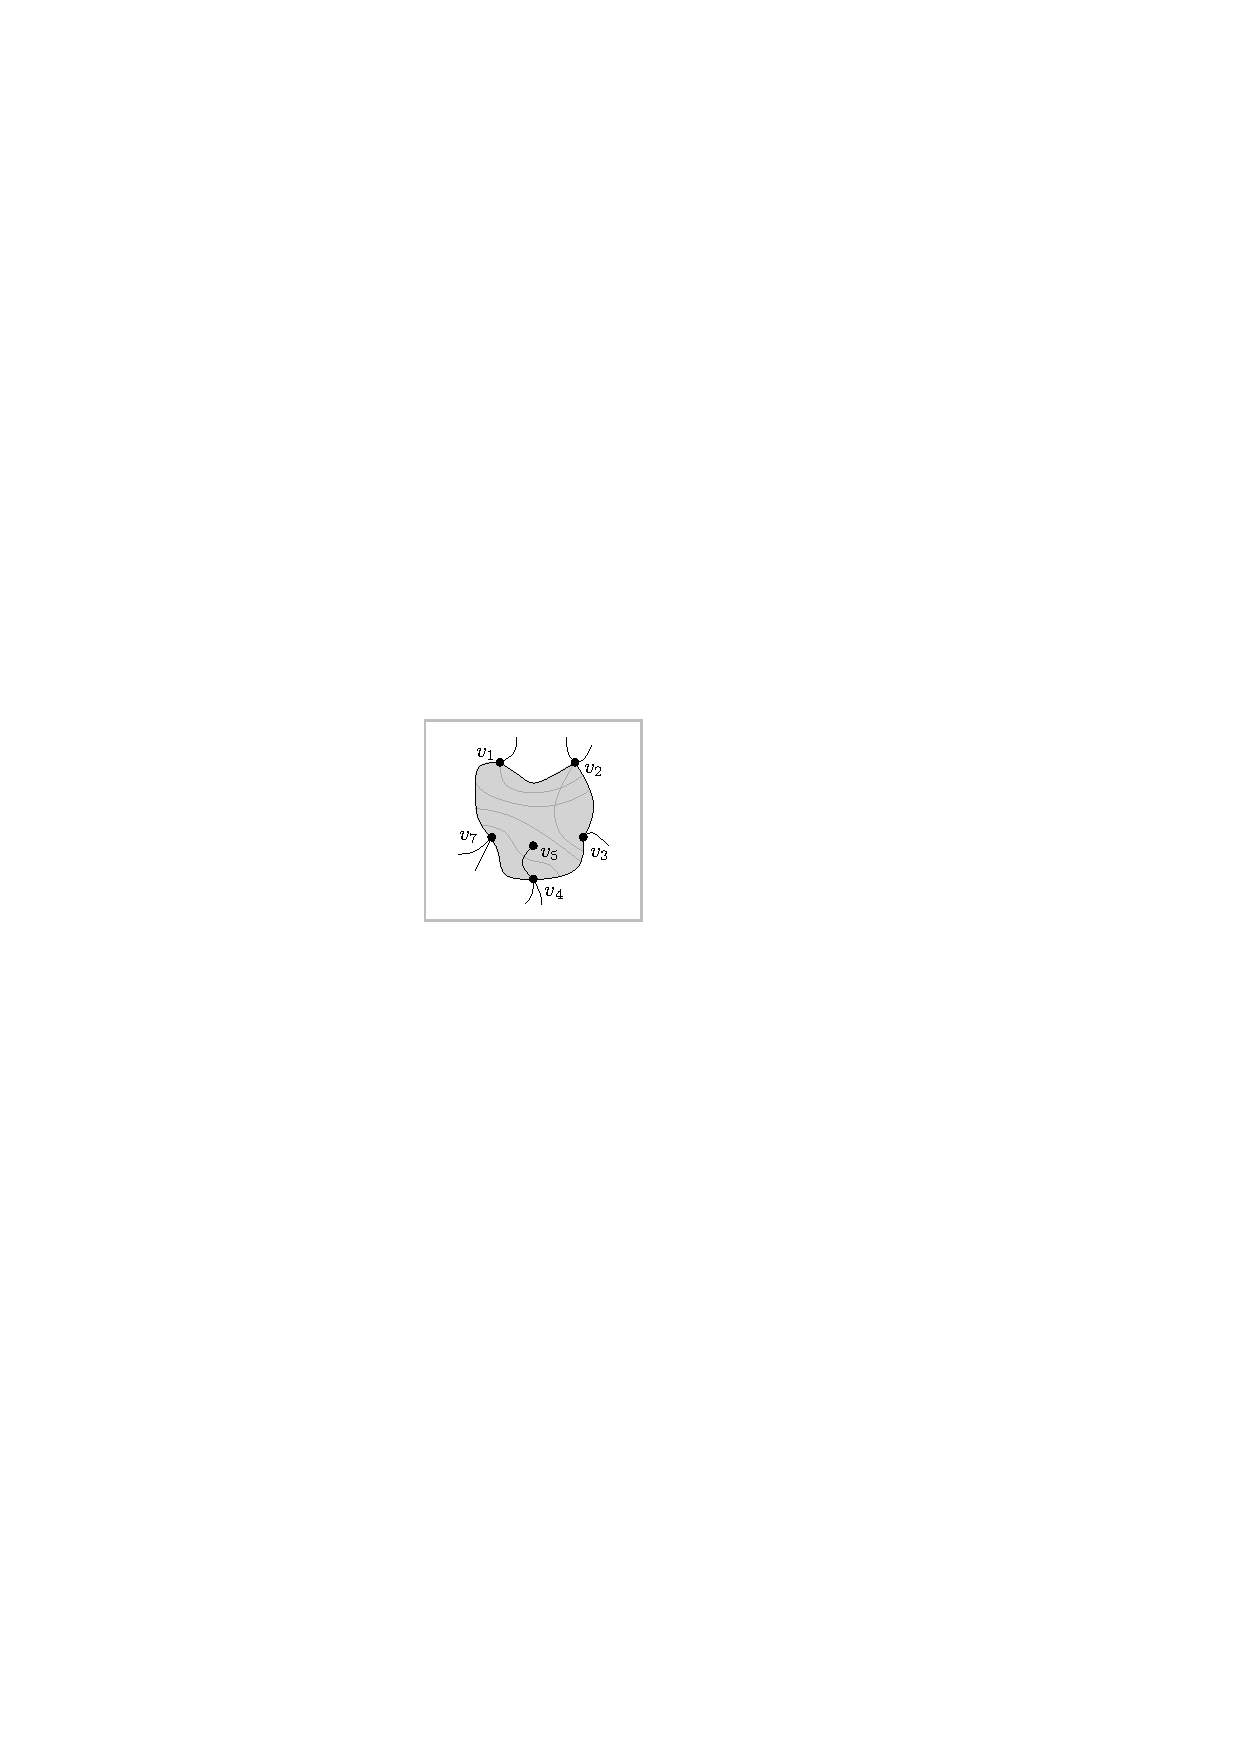
\includegraphics[width=\textwidth,page=1]{images/preliminaries}
        \subcaption{~}\label{fig:non_simple_face}
    \end{minipage}
	\begin{minipage}[b]{.18\textwidth}
        \centering
        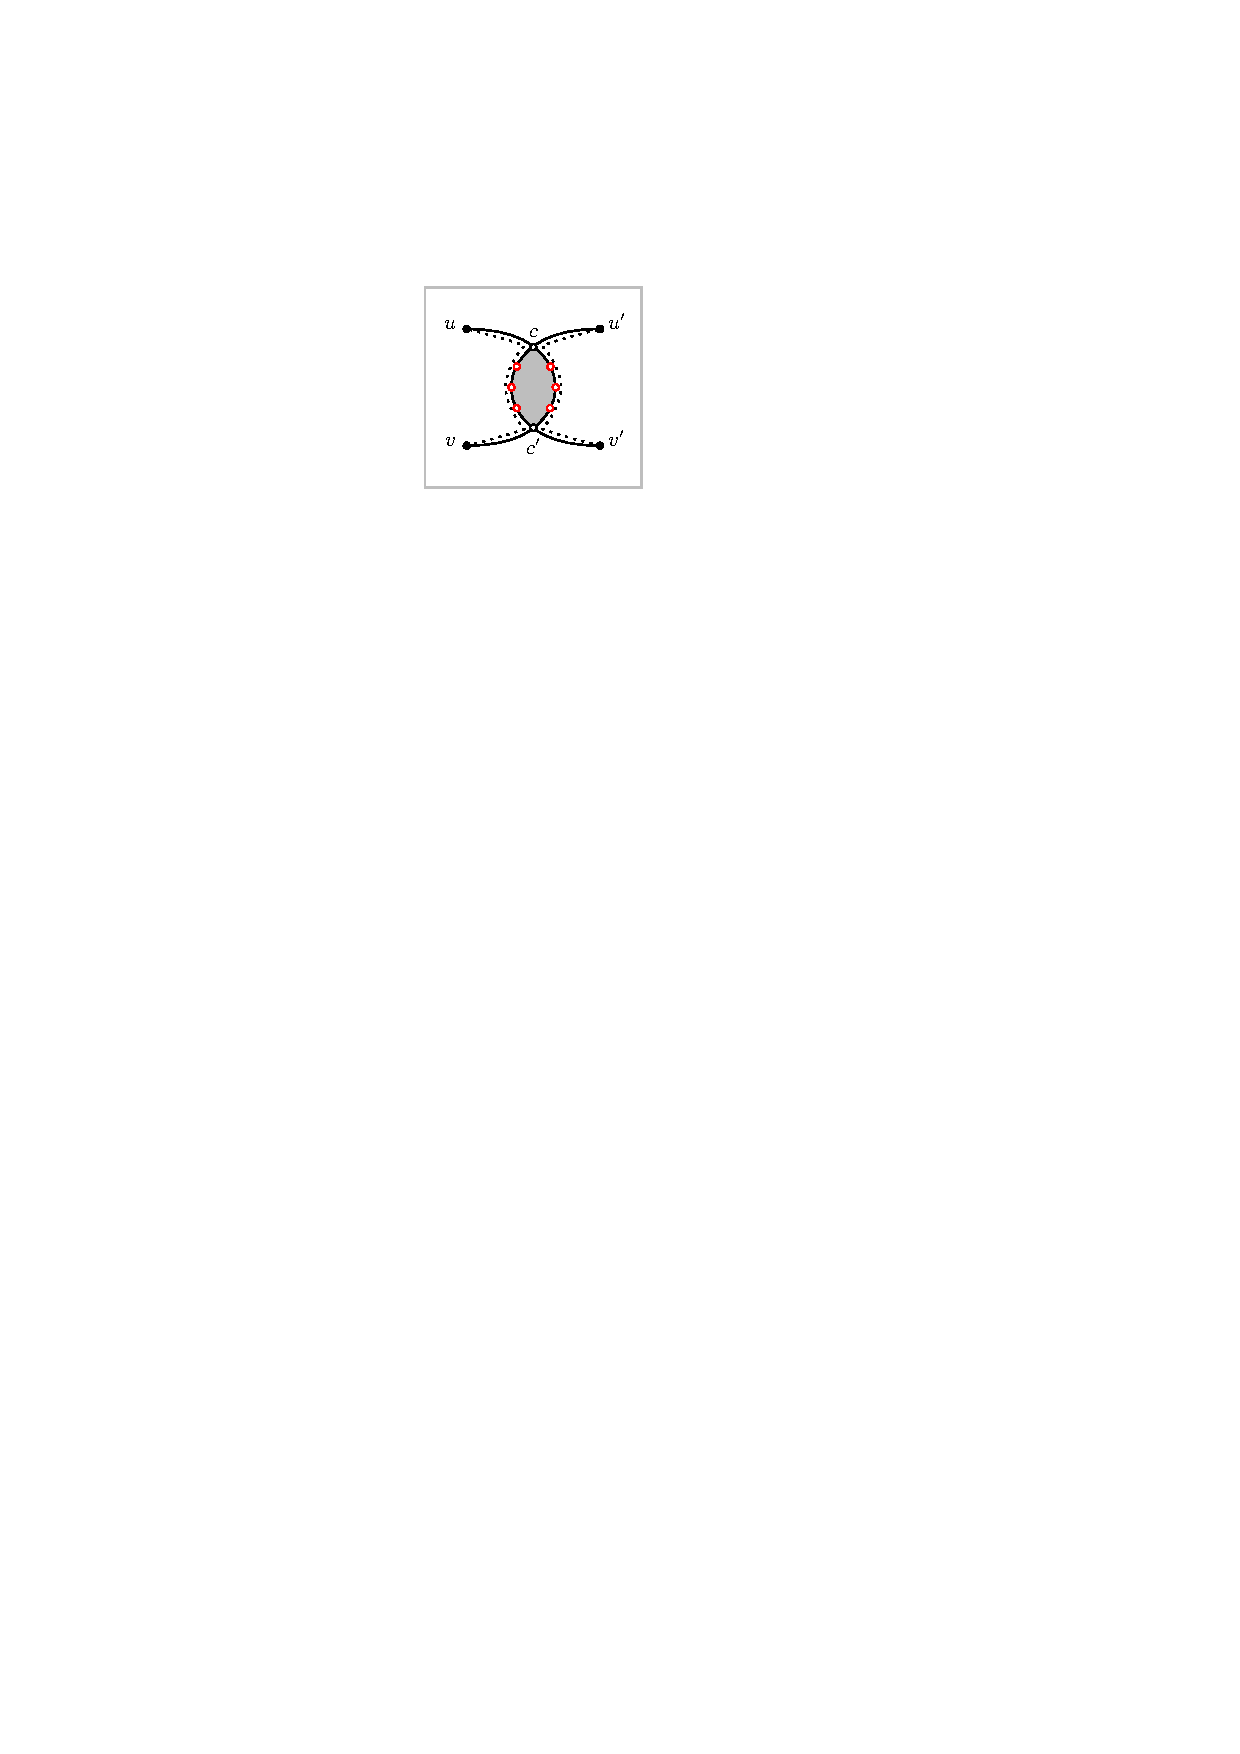
\includegraphics[width=\textwidth,page=1]{images/crossing_conf}
        \subcaption{~}\label{fig:crossing_twice}
    \end{minipage}	
    \begin{minipage}[b]{.18\textwidth}
        \centering
        \includegraphics[width=\textwidth,page=2]{images/crossing_conf}
        \subcaption{~}\label{fig:crossing_twice_2}
    \end{minipage}
    \begin{minipage}[b]{.18\textwidth}
        \centering
        \includegraphics[width=\textwidth,page=3]{images/crossing_conf}
        \subcaption{~}\label{fig:crossing_adjacent}
    \end{minipage}	
    \begin{minipage}[b]{.18\textwidth}
        \centering
        \includegraphics[width=\textwidth,page=4]{images/crossing_conf}
        \subcaption{~}\label{fig:crossing_adjacent_2}
    \end{minipage}	
    \caption{%
    (a)~A non-simple face $\{v_1,\ldots,v_7\}$, where $v_6$ is identified with $v_4$.
    Different configurations used in 
    (b-c)~Lemma~\ref{lem:crossing_twice}, and 
    (d-e)~Lemma~\ref{lem:crossing_adjacent}.}
    \label{fig:2_planar_polygon_conf}
\end{figure} 

Drawing $\Gamma(G)$ is called \emph{$k$-planar} if every edge in $\Gamma(G)$ is crossed at most $k$ times. Accordingly, a graph is called \emph{$k$-planar} if it admits a $k$-planar drawing. An \emph{optimal $k$-planar} graph is a $k$-planar graph with the maximum number of edges (e.g., an optimal $1$-planar graph on $n$ vertices is a $1$-planar graph with exactly $4n-8$ edges). For an optinal $k$-planar graph $G$ on $n$ vertices, a $k$-planar drawing $\Gamma(G)$ of $G$ is called \emph{planar-maximal crossing-minimal} or simply PMCM-drawing if and only if $\Gamma(G)$ has the maximum number of true-planar edges among all $k$-planar drawings of $G$ and, subject to this restriction, $\Gamma(G)$ has also the minimum number of crossings.

\begin{lemma}
Let $\Gamma(G)$ be a PMCM-drawing of an optimal $k$-planar graph $G$ in which two edges $(u,v)$ and $(u',v')$ cross more that once. Let $c$ and $c'$ be two consecutive crossing points of them. Then, the closed region $R_{c,c'}$ that is defined by $(u,v)$, $(u',v')$ and the crossing points $c$ and $c'$ has at least one vertex in its interior.
\label{lem:crossing_twice}
\end{lemma}
\begin{proof}
For a proof by contradiction, assume that there is no vertex in $R_{c,c'}$. Denote by $nc(u,v)$ and $nc(u',v')$ the number of crossings along $(u,v)$ and $(u',v')$ that are between $c$ and $c'$, respectively (red drawn in Figure~\ref{fig:crossing_twice}). First assume that $nc(u,v) = nc(u',v')$. We will cope with the case where $nc(u,v) \neq nc(u',v')$ shortly. We proceed by redrawing edge $(u,v)$ and $(u',v')$ so to eliminate both crossings $c$ and $c'$ without affecting the $k$-planarity of $G$; see the dotted-drawn edges of Figure~\ref{fig:crossing_twice}. Of course, this contradicts the crossing minimality of $\Gamma(G)$. To complete the proof of this lemma, it remains to consider the case where $nc(u,v) \neq nc(u',v')$. Assume w.l.o.g.~that $nc(u,v) > nc(u',v')$. In this case, there is at least one other edge, say $(u'',v'')$, that crosses $(u,v)$ between $c$ and $c'$ at least twice, say at points $d$ and $d'$; refer to Figure~\ref{fig:crossing_twice_2}. Since the ``length'' between $d$ and $d'$ is shorter than the length between $c$ and $c'$, it follows that if we apply the analysis above on $(u,v)$ and $(u'',v'')$, then there will be eventually a pair of crossing edges, say $e$ and $e'$, that will have exactly the same number of crossings, that is, $nc(e) = nc(e')$. This pair of edges contradicts the crossing minimality of $\Gamma(G)$.    
\end{proof}
 

\begin{lemma}
Let $\Gamma(G)$ be a PMCM-drawing of an optimal $k$-planar graph $G$ in which two edges $(u,v)$ and $(u,v')$ incident to a common vertex $u$ cross. Let $c$ be the first crossing point of $(u,v)$ with $(u,v')$ starting from $u$. Then, the closed region $R_{c}$ that is defined by vertex $u$, edges $(u,v)$, $(u,v')$ and $c$ has at least one vertex in its interior.
\label{lem:crossing_adjacent}
\end{lemma}
\begin{proof}
For a proof by contradiction, assume that there is no vertex in $R_{c}$. Denote by $nc(u,v)$ and $nc(u,v')$ the number of crossings along $(u,v)$ and $(u,v')$ that are between $u$ and $c$, respectively (red drawn in Figure~\ref{fig:crossing_twice_2}). First assume that $nc(u,v) = nc(u,v')$. We will cope with the case where $nc(u,v) \neq nc(u,v')$ shortly. We proceed by eliminating crossing $c$ without affecting the $k$-planarity of $G$; see the dotted-drawn edges of Figure~\ref{fig:crossing_adjacent}. Of course, this contradicts the crossing minimality of $\Gamma(G)$. To complete the proof of this property, it remains to consider the case where $nc(u,v) \neq nc(u,v')$. Assume w.l.o.g.~that $nc(u,v) > nc(u,v')$. In this case, there is either one other edge of $u$, say $(u,v'')$ that crosses $(u,v)$ between $u$ and $c$, or there exists an edge $(u'',v'')$ that crosses at least twice edge $(u,v)$. By Lemma~\ref{lem:crossing_twice}, the latter case would imply that $R_{c}$ is not an empty region; a contradiction. Hence, there exists at least one other edge, say $(u,v'')$, that crosses $(u,v)$ between $u$ and $c$, say at point $d$; refer to Figure~\ref{fig:crossing_adjacent_2}. Since the ``length'' between $u$ and $d$ is shorter than the length between $u$ and $c$, it follows that if we apply the analysis above on $(u,v)$ and $(u,v'')$, then there will be eventually a pair of crossing edges incident to $u$, say $e$ and $e'$ that have exactly the same number of crossings, that is, $nc(e) = nc(e')$. This pair of edges contradicts the crossing minimality of $\Gamma(G)$.   
\end{proof}

A Jordan curve $[u,v]$ joining vertices $u$ and $v$ of $G$ is a \emph{\pe} in drawing $\Gamma(G)$ if and only if $[u,v]$ is not a homotopic self-loop in $\Gamma(G)$, that is, either $u \neq v$ or $u=v$ and there is at least one vertex in the interior and the exterior of $[u,v]$. Note that $u$ and $v$ are not necessarily adjacent in $G$. However, since each topological edge $(u,v) \in E$ of $G$ is represented by a Jordan curve in $\Gamma(G)$, it follows that $(u,v)$ is by definition a \pe of $G$ (among other ones that can potentially exist).

We say that vertices $v_1,v_2,\dots,v_k$ define a \emph{\pp} in $\Gamma(G)$, if there exist \pes $[v_i,v_{i+1}]$, for $i=1,\dots, k-1$ and \pe $[v_1,v_k]$ of $\Gamma(G)$, which %
\begin{inparaenum}[(i)]
\item do not cross with each other and
\item define a region in $\Gamma(G)$ that has no vertices in its interior.
\end{inparaenum}
%
%We refer to the (empty of vertices) interior region of a \pp as a \emph{polygonal region} (denoted by $\mathcal{R}_k$), and to its boundary as a \emph{polygonal boundary} (denoted by $\mathcal{B}_k$).

Now, consider a pair of vertices $u$ and $v$ of $G$ that are not necessarily distinct. We say that $u$ and $v$ form a \emph{corner pair} if and only if an edge $(u,u')$ incident to $u$ crosses an edge $(v,v')$ incident to $v$ in $\Gamma(G)$; see Figure~\ref{fig:corner_pair}. Let $c$ be the crossing point of $(u,u')$ and $(v,v')$. Clearly, any Jordan curve $[u,v]$ joining vertices $u$ and $v$ defines a closed region $R_{u,v}$ with edge-segments $(u,c)$ and $(v,c)$. We call $[u,v]$ \emph{corner edge} w.r.t.~$(u,u')$ and $(v,v')$ if and only if $R_{u,v}$ has no vertices of $G$ in its interior.   

\begin{property}
In a PMCM-drawing $\Gamma(G)$ of an optimal $k$-planar graph $G$ any corner edge $[u,v]$ is a potential edge.
\label{prp:corner}
\end{property}
\begin{proof}
By the definition of potential edges, it follows that the property holds when $u \neq v$. Consider now the case where $u=v$. In this case $[u,v]$ is a self-loop; see Figure~\ref{fig:corner_pair_same}. If the property does not hold, then it follows that $[u,v]$ is a self-loop with no vertices either in its interior or in its exterior. The former case clearly contradicts Lemma~\ref{lem:crossing_adjacent}. So we may assume w.l.o.g.~that there is no vertex in the exterior of $[u,v]$; see Figure~\ref{fig:corner_pair_ext}. In this case, however, it follows that the two edges $(u,u')$ and $(v,v')$ defining $[u,v]$ must cross more than once in the exterior of $[u,v]$, which leads to a contradiction with Lemma~\ref{lem:crossing_adjacent}.
\end{proof}

 \begin{figure}[tb]
    \centering		
    \begin{minipage}[b]{.16\textwidth}
        \centering
        \includegraphics[width=\textwidth,page=2]{images/preliminaries}
        \subcaption{~}\label{fig:corner_pair}
    \end{minipage}
    \begin{minipage}[b]{.16\textwidth}
        \centering
        \includegraphics[width=\textwidth,page=3]{images/preliminaries}
        \subcaption{~}\label{fig:corner_pair_same}
    \end{minipage}
    \begin{minipage}[b]{.16\textwidth}
        \centering
        \includegraphics[width=\textwidth,page=4]{images/preliminaries}
        \subcaption{~}\label{fig:corner_pair_ext}
    \end{minipage}
    \begin{minipage}[b]{.16\textwidth}
        \centering
        \includegraphics[width=\textwidth,page=5]{images/preliminaries}
        \subcaption{~}\label{fig:parallel_pair}
    \end{minipage}
	\begin{minipage}[b]{.16\textwidth}
        \centering
        \includegraphics[width=\textwidth,page=6]{images/preliminaries}
        \subcaption{~}\label{fig:parallel_pair_same}
    \end{minipage}
	\begin{minipage}[b]{.16\textwidth}
        \centering
        \includegraphics[width=\textwidth,page=7]{images/preliminaries}
        \subcaption{~}\label{fig:parallel_pair_homotopic}
    \end{minipage}
    \caption{%    
    (a-c)~vertices $u$ and $v$ form a corner pair;
    (d-e)~vertices $u$ and $v$ form a parallel pair; 
    (f)~at least one of the two potential parallel edges exists.}
    \label{fig:crossing_confs}
\end{figure} 

We say that vertices $u$ and $v$ form a \emph{parallel pair} if and only if an edge $(u,u')$ of $u$ and an edge $(v,v')$ of $v$ both cross a third edge $(w,w')$ in $\Gamma(G)$ and additionally $(u,u')$ is not identified with $(v,v')$; see Figure~\ref{fig:parallel_pair}. Let $c$ and $c'$ be the crossing points of $(u,u')$ and $(v,v')$ with $(w,w')$, respectively. Clearly, any Jordan curve $[u,v]$ joining vertices $u$ and $v$ defines a closed region $R_{u,v}$ with edge-segments $(u,c)$, $(c,c')$ and $(v,c')$. We call $[u,v]$ \emph{parallel edge} w.r.t.~$(u,u')$ and $(v,v')$ if and only if $R_{u,v}$ has no vertices of $G$ in its interior. Symmetrically we define region $R_{u',v'}$ and parallel edge $[u',v']$ w.r.t.~$(u,u')$ and $(v,v')$.

%We denote a corner (parallel) pair formed by $u$ and $v$ by $\ppp{u}{v}$ ($\ppc{u}{v}$, resp.). We have the following properties:

\begin{property}
In a PMCM-drawing $\Gamma(G)$ of an optimal $k$-planar graph $G$ at least one of parallel edges $[u,v]$, $[u',v']$ is a potential edge.
\label{prp:parallel}
\end{property}
\begin{proof}
For a proof by contradiction, assume that neither $[u,v]$ nor $[u',v']$ is a potential edge. This implies that $u=v$, $u'=v'$ and both $[u,v]$ and $[u',v']$ are self-loops that have no vertices in their interiors or their exteriors. Figure~\ref{fig:parallel_pair_homotopic} illustrates the case where both $[u,v]$ and $[u',v']$ are self-loops with no vertices in their interiors; the other cases are symmetric. It is not hard to see that $(u,u')$ and $(v,v')$ are homotopic parallel edges; a contradiction.
\end{proof}
%
We say that $(u,u')$ and $(v,v')$ are \emph{independent} if and only if both parallel edges $[u,v]$ and $[u',v']$ are \pes.

\begin{remark}
Note that in the definition of parallel pairs we required $(u,u')$ not to be identified with $(v,v')$. If this is not the case, then edge $(w,w')$ is being crossed twice by $(u,u') = (v,v')$. To make the description of our proofs simple, in Sections~\ref{sec:2planar} and \ref{sec:3planar} we will initially require that every pair of edges in $\Gamma(G)$ crosses at most once. We will call a drawing fulfilling this requirement \emph{almost-simple}. This requirement will be formally proved in both cases (see Lemmas~\ref{lem:2_planar_cross_twice} and~\ref{lem:3_planar_cross_twice}).    
\end{remark}




\input{properties.tex}
% ============================================================================
\section{Characterization of 2-planar graphs}
\label{sec:2planar}
% ============================================================================

Let $G$ be an optimal $2$-planar graph on $n$ vertices (and therefore with $5n-10$ edges). Let also $\Gamma(G)$ be a PMCM $2$-planar drawing of $G$, i.e. $\Gamma(G)$ has the maximum number of true-planar edges among all potential $2$-planar drawing of $G$ and, subject to this restriction, $\Gamma(G)$ has also the minimum number of crossings. For the sake of simplicity we also momentarily assume that in $\Gamma(G)$ there is no pair of edges that cross twice, i.e. $\Gamma(G)$ is almost-simple. This assumption  will be settled soon (see Lemma~\ref{lem:2_planar_cross_twice}). In the following lemmas, we examine structural properties of an almost-simple PMCM-drawing $\Gamma(G)$.

Note that in an almost-simple PMCM-drawing $\Gamma(G)$, whenever edge $(w,w')$ has at least $2$ crossings, say $c$ and $c'$, then there exist two (non identical) edges $(u,u')$ and $(v,v')$ that cross $(w,w')$ at $c$ and $c'$ respectively. This implies that vertices $u$ and $v$ always form a parallel pair, and so do vertices $u'$ and $v'$. Since this property will be heavily used throughout the paper, we shall not explicitly state it every time, but rather implicitly imply it.

%\todo[inline]{add in every lemma the assumption about edges crossing twice}

\begin{lemma}
Let $\Gamma(G)$ be an almost-simple PMCM $2$-planar drawing of an optimal $2$-planar graph $G$ on $n$ vertices. Any edge that is crossed twice in  $\Gamma(G)$ is a chord of a true-planar $5$-cycle in $\Gamma(G)$. 
\label{lem:2_planar_small_faces}
\end{lemma}

\begin{proof}
Let $(w,w')$ be an edge of $G$ that is crossed twice in $\Gamma(G)$ and let $(u,u')$ and $(v,v')$ be the corresponding edges crossed by $(w,w')$. This crossing configuration defines four corner pairs: $\{w,u\}$, $\{w,u'\}$, $\{w,v\}$, $\{w,v'\}$, and two parallel pairs: $\{u,v\}$ and $\{u',v'\}$. By Lemmas~\ref{lem:crossing_twice} and ~\ref{lem:crossing_adjacent}, all corner edges are \pes, and either one or two of the parallel edges are \pes. We distinguish two cases depending on whether both parallel edges are \pes or not.

%Let $(u,v)$ be an edge of $G$ that is crossed twice in $\Gamma(G)$ and let $(u_1,v_1)$ and $(u_2,v_2)$ be the corresponding edges crossed by $(u,v)$. This crossing configuration defines four corner pairs: $\{u,u_1\}$, $\{u,v_1\}$, $\{v,u_2\}$, $\{v,v_2\}$, and two parallel pairs: $\{u_1,u_2\}$ and $\{v_1,v_2\}$. By P.\ref{prop_corner} and P.\ref{prop_parallel}, all the potential corner edges exist, and there exists either one or two of the potential parallel edges. We distinguish two cases depending on whether there exist both potential parallel edges or not.

So suppose first, that both parallel edges $(u,v)$ and $(u',v')$ are \pes, as in Figure~\ref{fig:2_planar_both_parallel_before}. Then vertices $w,u,v,w',v',u'$ define a \pp $\mathcal{P}_6$ of six vertices (grey shaded in Figure~\ref{fig:2_planar_both_parallel_before}). The \pr $\mathcal{R}_6$ of $\mathcal{P}_6$ contains no vertices in its interior, and at most five edges of $\Gamma(G)$ pass through $\mathcal{R}_6$: edges $(w,w')$, $(u,u')$, $(v,v')$ and at most two other edges that cross $(u,u')$ or $(v,v')$. Note that since the \pr is an open topological region without vertices in its interior, there can not be an edge that lies entirely in its interior. We proceed by removing  edges $(w,w')$, $(u,u')$, $(v,v')$ and all other edges that cross $(u,u')$ or $(v,v')$, and replace them with the $2$-planar pattern of Figure~\ref{fig:2_planar_both_parallel_after}. In the derived graph there exist $6$ edges drawn in $\mathcal{R}_6$ and do not cross the boundary of the \pp. Hence, the derived graph has more edges than $G$; a contradiction to the optimality of $G$. Note that even in the case where the \pp is not simple, i.e. the vertices that define its boundary are not all distinct, the above argument still holds, as can be seen for example in Figure~\ref{fig:2_planar_both_parallel_non_simple}, where $w=u$ and $v=v'$.
\todo{fix the figure}
%So suppose first, that both potential parallel edges $(u_1,u_2)$ and $(v_1,v_2)$ exist, as in Figure~\ref{fig:2_planar_both_parallel_before}. Then vertices $u,u_1,u_2,v,v_2,v_1$ define a \pp $\mathcal{P}_6$ of six vertices (grey shaded in Figure~\ref{fig:2_planar_both_parallel_before}). The polygonal region $\mathcal{R}_6$ of $\mathcal{P}_6$ contains no vertices in its interior, and at most five edges of $\Gamma(G)$ pass through $\mathcal{R}_6$: edges $(u,v)$, $(u_1,v_1)$, $(u_2,v_2)$ and at most two other edges that cross $(u_1,v_1)$ or $(u_2,v_2)$. Note that since the polygonal region is an open topological region without vertices in its interior, there can not be an edge that lies entirely in its interior. We proceed by removing  edges $(u,v)$, $(u_1,v_1)$, $(u_2,v_2)$ and all other edges that cross $(u_1,v_1)$ or $(u_2,v_2)$, and replace them with the $2$-planar pattern of Figure~\ref{fig:2_planar_both_parallel_after}. In the derived graph there exist $6$ edges drawn in $\mathcal{R}_6$ and do not cross the boundary of the \pp. Hence, the derived graph has more edges than $G$; a contradiction to the optimality of $G$. Note that even in the case where the \pp is not simple, i.e. the vertices that define its boundary are not all distinct, the above argument still holds, as can be seen for example in Figure~\ref{fig:2_planar_both_parallel_non_simple}, where $u=u_1$ and $v_1=v_2$.

Suppose now that parallel edge $(u,v)$ is not a \pe. Then, it is $u=v$; refer to Figure~\ref{fig:2_planar_one_parallel_before}. This time, vertices $w,u,w',v',u'$ define a \pp $\mathcal{P}_5$ of five vertices (grey shaded in Figure~\ref{fig:2_planar_one_parallel_before}). As in the previous case, at most five edges of $\Gamma(G)$ pass through the polygonal region $\mathcal{R}_5$. We proceed by removing  edges $(w,w')$, $(u,u')$, $(v,v')$ and all other edges that cross $(u,u')$ or $(v,v')$, and replace them with the $2$-planar pattern of Figure~\ref{fig:2_planar_one_parallel_after}. In the derived graph there exist $5$ edges drawn in $\mathcal{R}_5$ plus the five \pes of the boundary of $\mathcal{P}_5$. Since $G$ is optimal, it follows that:
\begin{enumerate}
\item there exist exactly two edges other than $(w,w')$, say $e_1$ and $e_2$, that cross $(u,v)$ and $(u',v')$ respectively, and
\item  the \pes of the boundary of  $\mathcal{P}_5$ already exist in the drawing $\Gamma(G)$, i.e. $\mathcal{P}_5$ is a cycle, say $C$, of length $5$. 
\end{enumerate}

%Suppose now that potential parallel edge $(u_1,u_2)$ does not exist. Then, it is $u_1=u_2$; refer to Figure~\ref{fig:2_planar_one_parallel_before}. This time, vertices $u,u_1,v,v_2,v_1$ define a \pp $\mathcal{P}_5$ of five vertices (grey shaded in Figure~\ref{fig:2_planar_one_parallel_before}). As in the previous case, at most five edges of $\Gamma(G)$ pass through the polygonal region $\mathcal{R}_5$. We proceed by removing  edges $(u,v)$, $(u_1,v_1)$, $(u_1,v_2)$ and all other edges that cross $(u_1,v_1)$ or $(u_2,v_2)$, and replace them with the $2$-planar pattern of Figure~\ref{fig:2_planar_one_parallel_after}. In the derived graph there exist $5$ edges drawn in $\mathcal{R}_5$ plus the five \pes of the boundary of $\mathcal{P}_5$. Since $G$ is optimal, it follows that:
%\begin{enumerate}
%\item there exist exactly two edges other than $(u,v)$, say $e_1$ and $e_2$, that cross $(u_1,v_1)$ and $(u_1,v_2)$ respectively, and
%\item  the \pes of the boundary of  $\mathcal{P}_5$ already exist in the drawing $\Gamma(G)$, i.e. $\mathcal{P}_5$ is a cycle, say $C$, of length $5$. 
%\end{enumerate}

If $C$ is a true-planar $5$-cycle in $\Gamma(G)$ the lemma holds, so suppose that this is not the case. Then, at least one of edges $e_1$ or $e_2$ crosses $C$. Suppose w.l.o.g. that  edge $e_1=(w_1,w'_1)$ crosses edge $(v,v')$ of the $5$-cycle $C$ at crossing point $c$ (the case where $e_1$ crosses edge $(u,v)$ can be treated similarly);\todo{is it clear that it can't cross another edge of C?} refer to Figure~\ref{fig:2_planar_one_parallel_extra}. Note that $e_1$ already has two crossings in the drawing $\Gamma(G)$. Then, at least one of the edge segments $(w_1,c)$ or $(c,w'_1)$ of $e_1$ does not pass through the \pr $\mathcal{R}_5$. Suppose w.l.o.g. that this is edge segment $(w_1,c)$  of $e_1$. Then, vertices $w_1$ - $v$, and $w_1$ - $v'$ define two corner pairs of vertices. Hence vertices $w,u,w',v',w_1,v$ define a \pp $\mathcal{P}_6$ on six vertices, with exactly six edges passing through its \pr, say $\mathcal{R}_6$. We remove all edges that pass through $\mathcal{R}_6$ and replace it with the $2$-planar pattern of Figure~\ref{fig:2_planar_one_parallel_final}: we add one vertex and a total of $12$ edges. The derived graph, say $G'$, is $2$-planar and has $n'=n+1$ vertices and $m'=m+6$ edges (where $n$, $m$ are the number of vertices and edges of $G$ respectively). Hence $m'=5n'-9>5n'-10$, i.e. $G'$ has more edges than allowed; a contradiction.

%If $C$ is a true-planar $5$-cycle in $\Gamma(G)$ the lemma holds, so suppose that this is not the case. Then, at least one of edges $e_1$ or $e_2$ crosses $C$. Suppose w.l.o.g. that  edge $e_1=(w,w')$ crosses edge $(v_1,v_2)$ of the $5$-cycle $C$ at crossing point $c$ (the case where $e_1$ crosses edge $(u,v_1)$ can be treated similarly);\todo{is it clear that it can't cross another edge of C?} refer to Figure~\ref{fig:2_planar_one_parallel_extra}. Note that $e_1$ already has two crossings in the drawing $\Gamma(G)$. Then, at least one of the edge segments $(w,c)$ or $(c,w')$ of $e_1$ does not pass through the polygonal region $\mathcal{R}_5$. Suppose w.l.o.g. that this is edge segment $(w,c)$  of $e_1$. Then, vertices $w$ - $v_1$, and $w$ - $v_2$ define two corner pairs of vertices. Hence vertices $u,u_1,v,v_2,w,v_1$ define a polygonal region $\mathcal{P}_6$ on six vertices, with exactly six edges passing through its polygonal region, say $\mathcal{R}_6$. We remove all edges that pass through $\mathcal{R}_6$ and replace it with the $2$-planar pattern of Figure~\ref{fig:2_planar_one_parallel_final}: we add one vertex and a total of $12$ edges. The derived graph, say $G'$, is $2$-planar and has $n'=n+1$ vertices and $m'=m+6$ edges (where $n$, $m$ are the number of vertices and edges of $G$ respectively). Hence $m'=5n'-9>5n'-10$, i.e. $G'$ has more edges than allowed; a contradiction.\qed
\end{proof}

\begin{figure}[htb]
    \centering
    \begin{minipage}[b]{.24\textwidth}
        \centering
        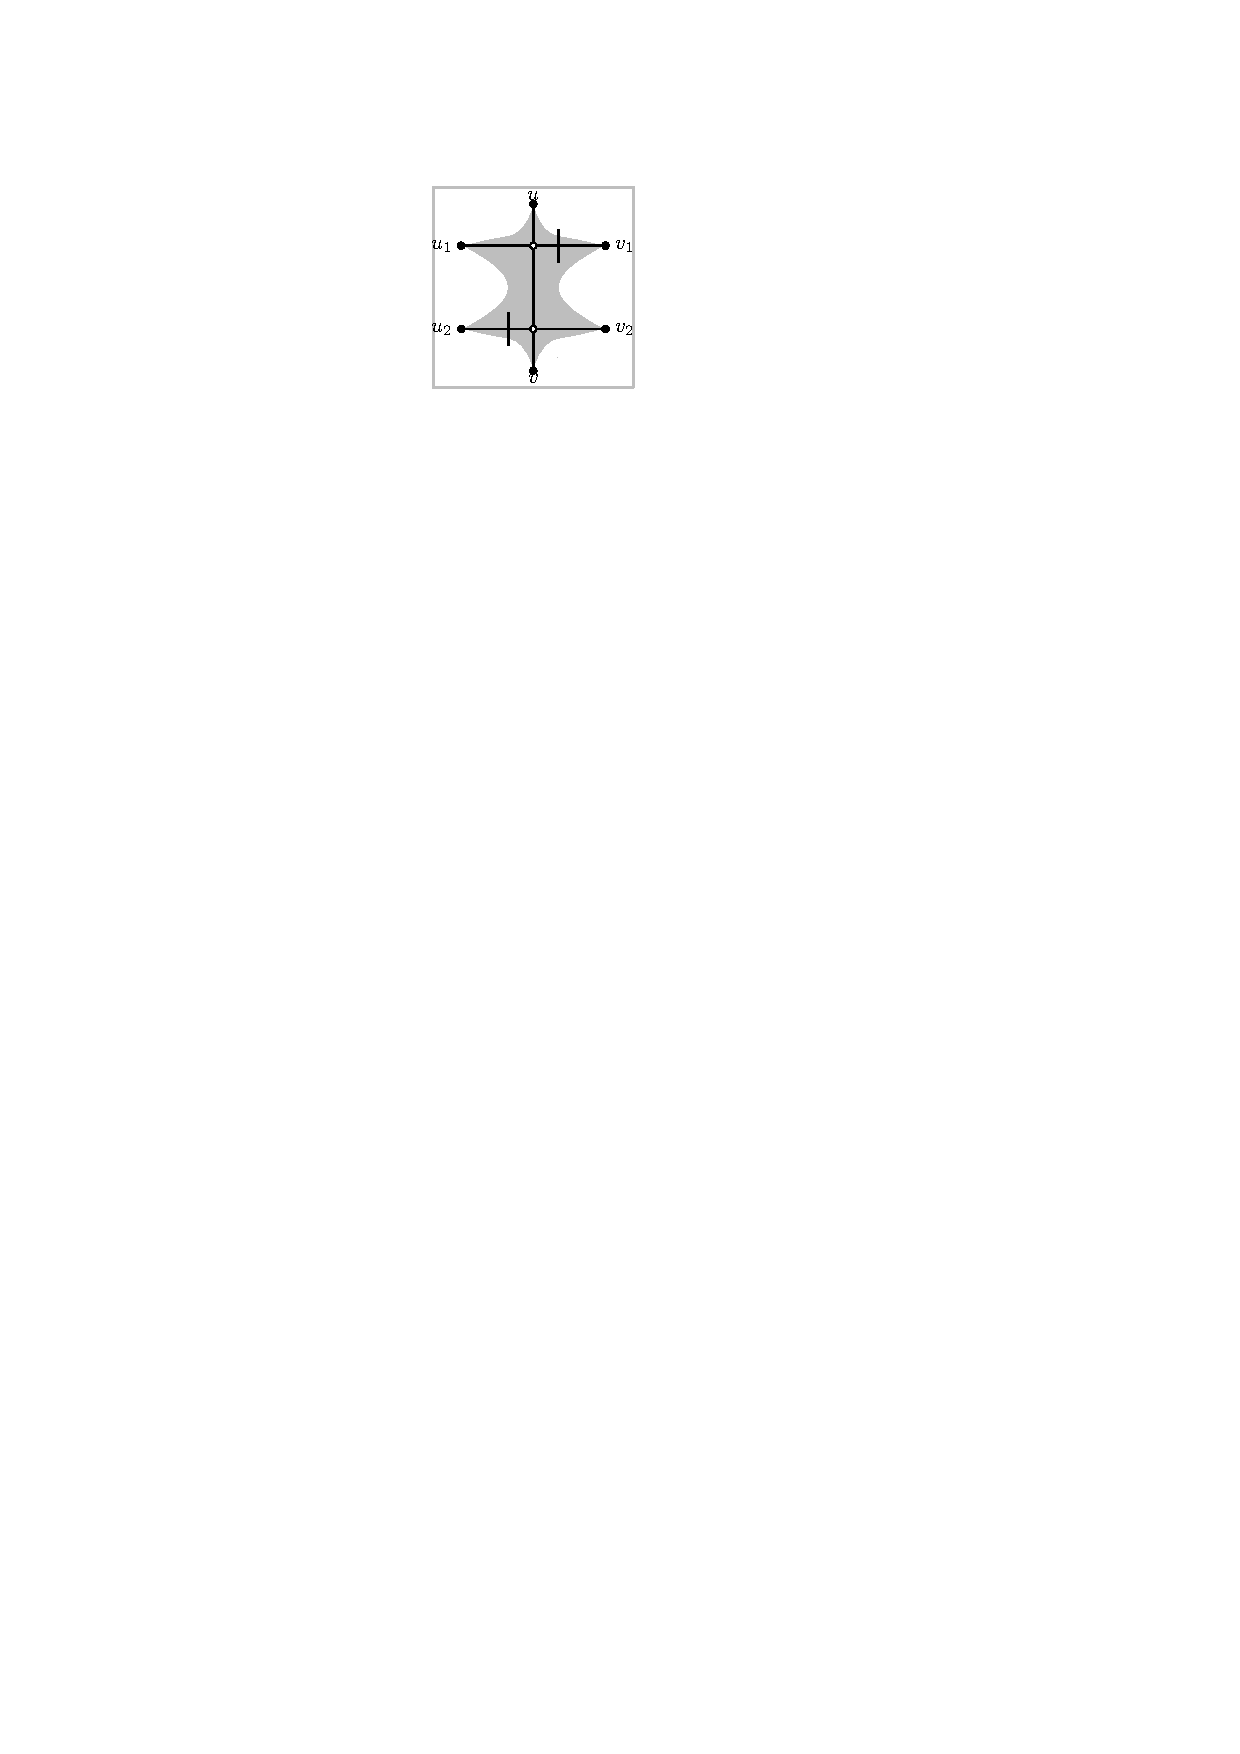
\includegraphics[width=\textwidth,page=1]{images/2_planar_potential_parallel}
        \subcaption{~}\label{fig:2_planar_both_parallel_before}
    \end{minipage}
    \begin{minipage}[b]{.24\textwidth}
        \centering
        \includegraphics[width=\textwidth,page=2]{images/2_planar_potential_parallel}
        \subcaption{~}\label{fig:2_planar_both_parallel_after}
    \end{minipage}
	\begin{minipage}[b]{.24\textwidth}
        \centering        
        \includegraphics[width=\textwidth,page=3]{images/2_planar_potential_parallel}
        \subcaption{~}\label{fig:2_planar_both_parallel_non_simple}
    \end{minipage}
		
    \begin{minipage}[b]{.24\textwidth}
        \centering
        \includegraphics[width=\textwidth,page=4]{images/2_planar_potential_parallel}
        \subcaption{~}\label{fig:2_planar_one_parallel_before}
    \end{minipage}
		\begin{minipage}[b]{.24\textwidth}
        \centering
        \includegraphics[width=\textwidth,page=5]{images/2_planar_potential_parallel}
        \subcaption{~}\label{fig:2_planar_one_parallel_after}
    \end{minipage}
		\begin{minipage}[b]{.24\textwidth}
        \centering
        \includegraphics[width=\textwidth,page=6]{images/2_planar_potential_parallel}
        \subcaption{~}\label{fig:2_planar_one_parallel_extra}
    \end{minipage}
		\begin{minipage}[b]{.24\textwidth}
        \centering
        \includegraphics[width=\textwidth,page=7]{images/2_planar_potential_parallel}
        \subcaption{~}\label{fig:2_planar_one_parallel_final}
    \end{minipage}
    \caption{%
    Different configurations used in Lemma~\ref{lem:2_planar_small_faces}.}
    \label{fig:2_planar_potential_parallel}
\end{figure}




By Lemma~\ref{lem:2_planar_small_faces}, we have that any edge of $G$ that is crossed twice in an almost-simple PMCM-drawing $\Gamma(G)$ is a chord of a true-planar $5$-cycle. So, it remains to consider edges of $G$ that have only one crossing in $\Gamma(G)$:

\begin{lemma}\label{lem:2_planar_one_crossing}
Let $\Gamma(G)$ be an almost-simple PMCM $2$-planar drawing of an optimal $2$-planar graph $G$ on $n$ vertices. Then every edge of $\Gamma(G)$ is either true-planar or has exactly two crossings.
\end{lemma}
\begin{proof}
By the proof of Lemma~\ref{lem:2_planar_small_faces}, we have that, for any edge of $G$ that is crossed twice in $\Gamma(G)$, both edges that cross this particular edge also have two crossing in $\Gamma(G)$. This implies that if edges $(u,u')$ and $(v,v')$ cross in $\Gamma(G)$ and $(u,u')$ has only one crossing, then the same holds for $(v,v')$. \todo{use propagated set}So, we have four corner pairs of  vertices: $u$ - $v$, $u$ - $v'$, $u'$ - $v$, $u'$ - $v'$, and all corner edges are \pes; refer to Figure~\ref{fig:2_planar_one_crossing_before}. Vertices  $u,v,v',u'$ define a \pp $\mathcal{P}_4$ of four vertices (grey shaded in Figure~\ref{fig:2_planar_one_crossing_before}). Since edges $(u,u')$ and $(v,v')$ have only one crossing each, the \pes of the boundary of $\mathcal{P}_4$ exist in $\Gamma(G)$ and are true-planar edges (Indeed if any of these \pes does not exist, one could add them in $\Gamma(G)$ without introducing any crossings or creating homotopic edges, contradicting the optimality of $G$). We proceed by removing  edges $(u,u')$ and $(v,v')$, and replace them with the $2$-planar pattern of Figure~\ref{fig:2_planar_one_crossing_after}. The derived graph, say $G'$ is $2$-planar and has $n'=n+2$ vertices and $m'=m+11$ edges (where $n$, $m$ are the number of vertices and edges of $G$ respectively). Hence $m'=5n'-9>5n'-10$, i.e. $G'$ has more edges than allowed; a contradiction.

%By the proof of Lemma~\ref{lem:2_planar_small_faces}, we have that, for any edge of $G$ that is crossed twice in $\Gamma(G)$, both edges that cross this particular edge also have two crossing in $\Gamma(G)$. This implies that if edges $(u_1,v_1)$ and $(u_2,v_2)$ cross in $\Gamma(G)$ and $(u_1,v_1)$ has only one crossing, then the same holds for $(u_2,v_2)$. So, we have four corner pairs of  vertices: $u_1$ - $u_2$, $u_1$ - $v_2$, $v_1$ - $u_2$, $v_1$ - $v_2$, and all the potential corner edges exist; refer to Figure~\ref{fig:2_planar_one_crossing_before}. Vertices  $u_1,u_2,v_2,v_1$ define a \pp $\mathcal{P}_4$ of four vertices (grey shaded in Figure~\ref{fig:2_planar_one_crossing_before}). Since edges $(u_1,v_1)$ and $(u_2,v_2)$ have only one crossing each, the \pes of the boundary of $\mathcal{P}_4$ exist in $\Gamma(G)$ and are true-planar edges (Indeed if any of these \pes does not exist, one could add them in $\Gamma(G)$ without introducing any crossings or creating homotopic edges, contradicting the optimality of $G$). We proceed by removing  edges $(u_1,v_1)$ and $(u_2,v_2)$, and replace them with the $2$-planar pattern of Figure~\ref{fig:2_planar_one_crossing_after}. The derived graph, say $G'$ is $2$-planar and has $n'=n+2$ vertices and $m'=m+11$ edges (where $n$, $m$ are the number of vertices and edges of $G$ respectively). Hence $m'=5n'-9>5n'-10$, i.e. $G'$ has more edges than allowed; a contradiction.\qed
\end{proof}


\begin{figure}[htb]
    \centering
    \begin{minipage}[b]{.24\textwidth}
        \centering
        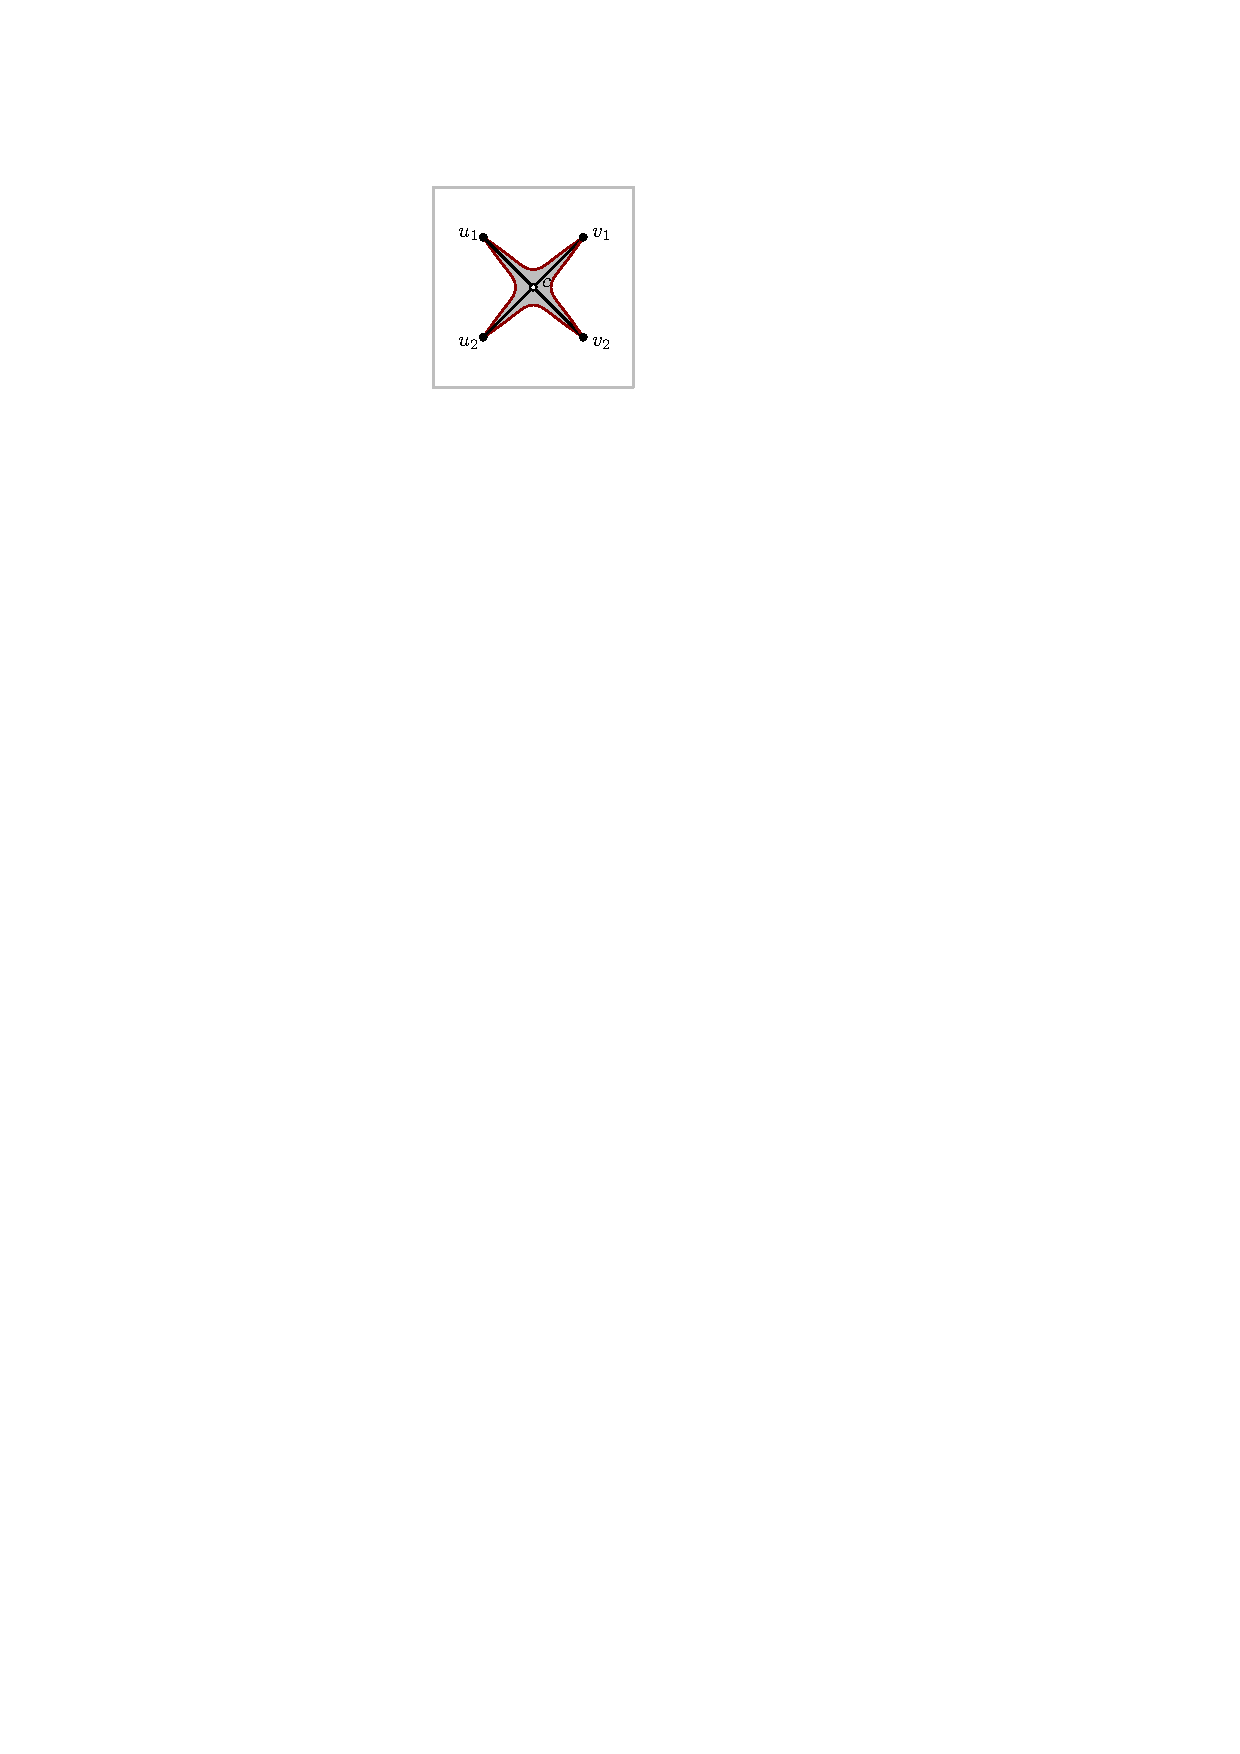
\includegraphics[width=\textwidth,page=1]{images/2planar_one_crossing}
        \subcaption{~}\label{fig:2_planar_one_crossing_before}
    \end{minipage}
    \begin{minipage}[b]{.24\textwidth}
        \centering
        \includegraphics[width=\textwidth,page=2]{images/2planar_one_crossing}
        \subcaption{~}\label{fig:2_planar_one_crossing_after}
    \end{minipage}
    \caption{%
    Configurations used in Lemma~\ref{lem:2_planar_one_crossing}}.
    \label{fig:2_planar_one_crossing}
\end{figure}

almost-simple PMCM
 
Now we are ready to prove the main property of every almost-simple PMCM-drawing $\Gamma(G)$ of a maximal $2$-planar graph. By Lemmas~\ref{lem:2_planar_small_faces} and \ref{lem:2_planar_one_crossing} we have that there exist only edges with two crossings and true-planar edges in $\Gamma(G)$ that create only true-planar $5$-cycles. Hence we have proven the following:
 
 %\todo[inline]{make lemma~\ref{lem:2_planar_faces} a corrolary}
 \begin{corollary}\label{cor:2_planar_faces}
  The true planar skeleton $\Pi(G)$ of an almost-simple PMCM-drawing $\Gamma(G)$ of a maximal $2$-planar graph $G$ contains only faces of length $5$.
 \end{corollary}
 %Now we are ready to prove the main property of maximal $2$-planar graphs. By Lemmas~\ref{lem:2_planar_small_faces} and \ref{lem:2_planar_one_crossing} we have that there exist only edges with two crossings and true-planar edges in $\Gamma(G)$ that create only $5$-cycles. Hence we have proven the following:
 %
 %\todo[inline]{make lemma~\ref{lem:2_planar_faces} a corrolary}
 %\begin{lemma}\label{lem:2_planar_faces}
  %The true planar subgraph $G_p$\todo{do we use true planar subgraph as notation?} contains only faces of length $5$.
 %\end{lemma}

Recall that at the beginning of this section we made the assumption that there is no pair of edges that cross twice in the drawing $\Gamma(G)$, i.e. that $\Gamma(G)$ is almost-simple. In the following, we prove that any PMCM-drawing of a maximal $2$-planar graph is almost-simple.
%Recall that at the beginning of this section we made the assumption that there is no pair of edges that cross twice in the drawing $\Gamma(G)$. In the following, we prove that in a planar-maximal crossing-minimal drawing there are no such pairs of edges.



%\begin{lemma}
%Let $\Gamma(G)$ be a $2$-planar drawing of an optimal $2$-planar graph $G$ on $n$ vertices. There is no pair of edges that cross twice in $\Gamma(G)$. 
%\label{lem:2_planar_cross_twice}
%\end{lemma}
%
%\begin{proof}
%Suppose that there exist edges $(u_1,v_1)$ and $(u_2,v_2)$ that cross twice at crossing points $c_1$ and $c_2$. Consider the bounded region $R$ defined by $(c_1,c_2)$ segment of edges $(u_1,v_1)$ and $(u_2,v_2)$. Since edges $(u_1,v_1)$ and $(u_2,v_2)$ both have two crossings, no other edge of $G$ crosses the boundary of $R$. Hence, if there exists at least one vertex of $G$ inside this region, $G$ is not connected; a contradiction.\todo{mention that G is connected} On the other hand, if $R$ is empty, we could redraw edges $(u_1,v_1)$ and $(u_2,v_2)$ so that they do not cross; a contradiction to the fact that $\Gamma(G)$ is crossing-minimal.\qed
%\end{proof}

By combining Lemmas~\ref{lem:2_planar_faces} and \ref{lem:2_planar_cross_twice}, we can characterize all optimal $2$-planar graphs:


 By Lemma~\ref{lem:2_planar_cross_twice} we have that Lemma~\ref{lem:2_planar_faces} holds for all maximal $2$-planar graphs. Since the true planar skeleton of such a graph contains only faces of length $5$, we can start with a $5$-tiling of the plane\todo{rephrase}. Now in the interior of every face of length $5$, we can add all  $5$ missing edges using the $2$-planar pattern of Figure~\ref{fig:2_planar_one_parallel_after}.


\section{Characterization of 3-planar graphs}
\label{sec:3planar}

%\todo[inline]{true planar subgraph or true planar skeleton?}
%\todo[inline]{change maximal to optimal}
Let $G$ be an optimal $3$-planar graph on $n$ vertices (and therefore with $5.5n-11$ edges) and let $\Gamma(G)$ be a PMCM $3$-planar drawing of $G$, i.e. $\Gamma(G)$ has the maximum number of true-planar edges among all potential $3$-planar drawing of $G$ and, subject to this restriction, $\Gamma(G)$ has also the minimum number of crossings. 
For the sake of simplicity we also assume that in the drawing $\Gamma(G)$ there is no pair of edges that cross twice, i.e. $\Gamma(G)$ is almost-simple. The assumption  will be settled  by Lemma~\ref{lem:3_planar_cross_twice}. In the following we examine structural properties of the almost-simple PMCM drawing $\Gamma(G)$, in particular we show  that the true planar skeleton$\Pi(G)$ of $\Gamma(G)$ consists of faces of length at most $9$. 
%The following lemmas describe some structural properties of $\Gamma(G)$.
%\todo[inline]{add in every lemma the assumption about edges crossing twice}


\begin{lemma}\label{lem:3_planar_true_planar}
Let $\Gamma(G)$ be a PMCM $3$-planar drawing of an optimal $3$-planar graph $G$ on $n$ vertices.
\begin{enumerate}
\item A true planar $6$-cycle in $\Gamma(G)$ without vertices in its interior, can not contain more than  $8$ chords in its interior; refer to Figure~\ref{fig:3_planar_polygon_conf_6}.
\item A true planar $7$-cycle in $\Gamma(G)$ without vertices in its interior, can not contain more than $9$ chords in its interior; refer to Figure~\ref{fig:3_planar_polygon_conf_7}.
\item A true planar $8$-cycle in $\Gamma(G)$ without vertices in its interior, can not contain more than $11$ chords in its interior; refer to Figure~\ref{fig:3_planar_polygon_conf_8}.
\item A true planar $9$-cycle in $\Gamma(G)$ without vertices in its interior, can not contain more than $14$ chords in its interior; refer to Figure~\ref{fig:3_planar_polygon_conf_9}.
\item A true planar $10$-cycle in $\Gamma(G)$ without vertices in its interior, can not contain more than $17$ chords in its interior; refer to Figure~\ref{fig:3_planar_polygon_conf_10}.
\item A $7$-cycle in $\Gamma(G)$ with exactly one edge crossing its boundary can contain at least $10$ edges: $9$ chords in its interior  and an edge that crosses its boundary (with one crossing); refer to Figure~\ref{fig:3_planar_polygon_conf_7_stick}.
\item A $8$-cycle in $\Gamma(G)$ with exactly one edge crossing its boundary can contain at least $12$ edges: $11$ chords in its interior and an edge that crosses its boundary (with two crossings); refer to Figure~\ref{fig:3_planar_polygon_conf_8_stick}.
\end{enumerate}
\end{lemma}
\begin{proof}
The proof of this lemma is omitted as it can be checked exhaustively.
\end{proof}

\begin{figure}[htb]
    \centering
    \begin{minipage}[b]{.24\textwidth}
        \centering
        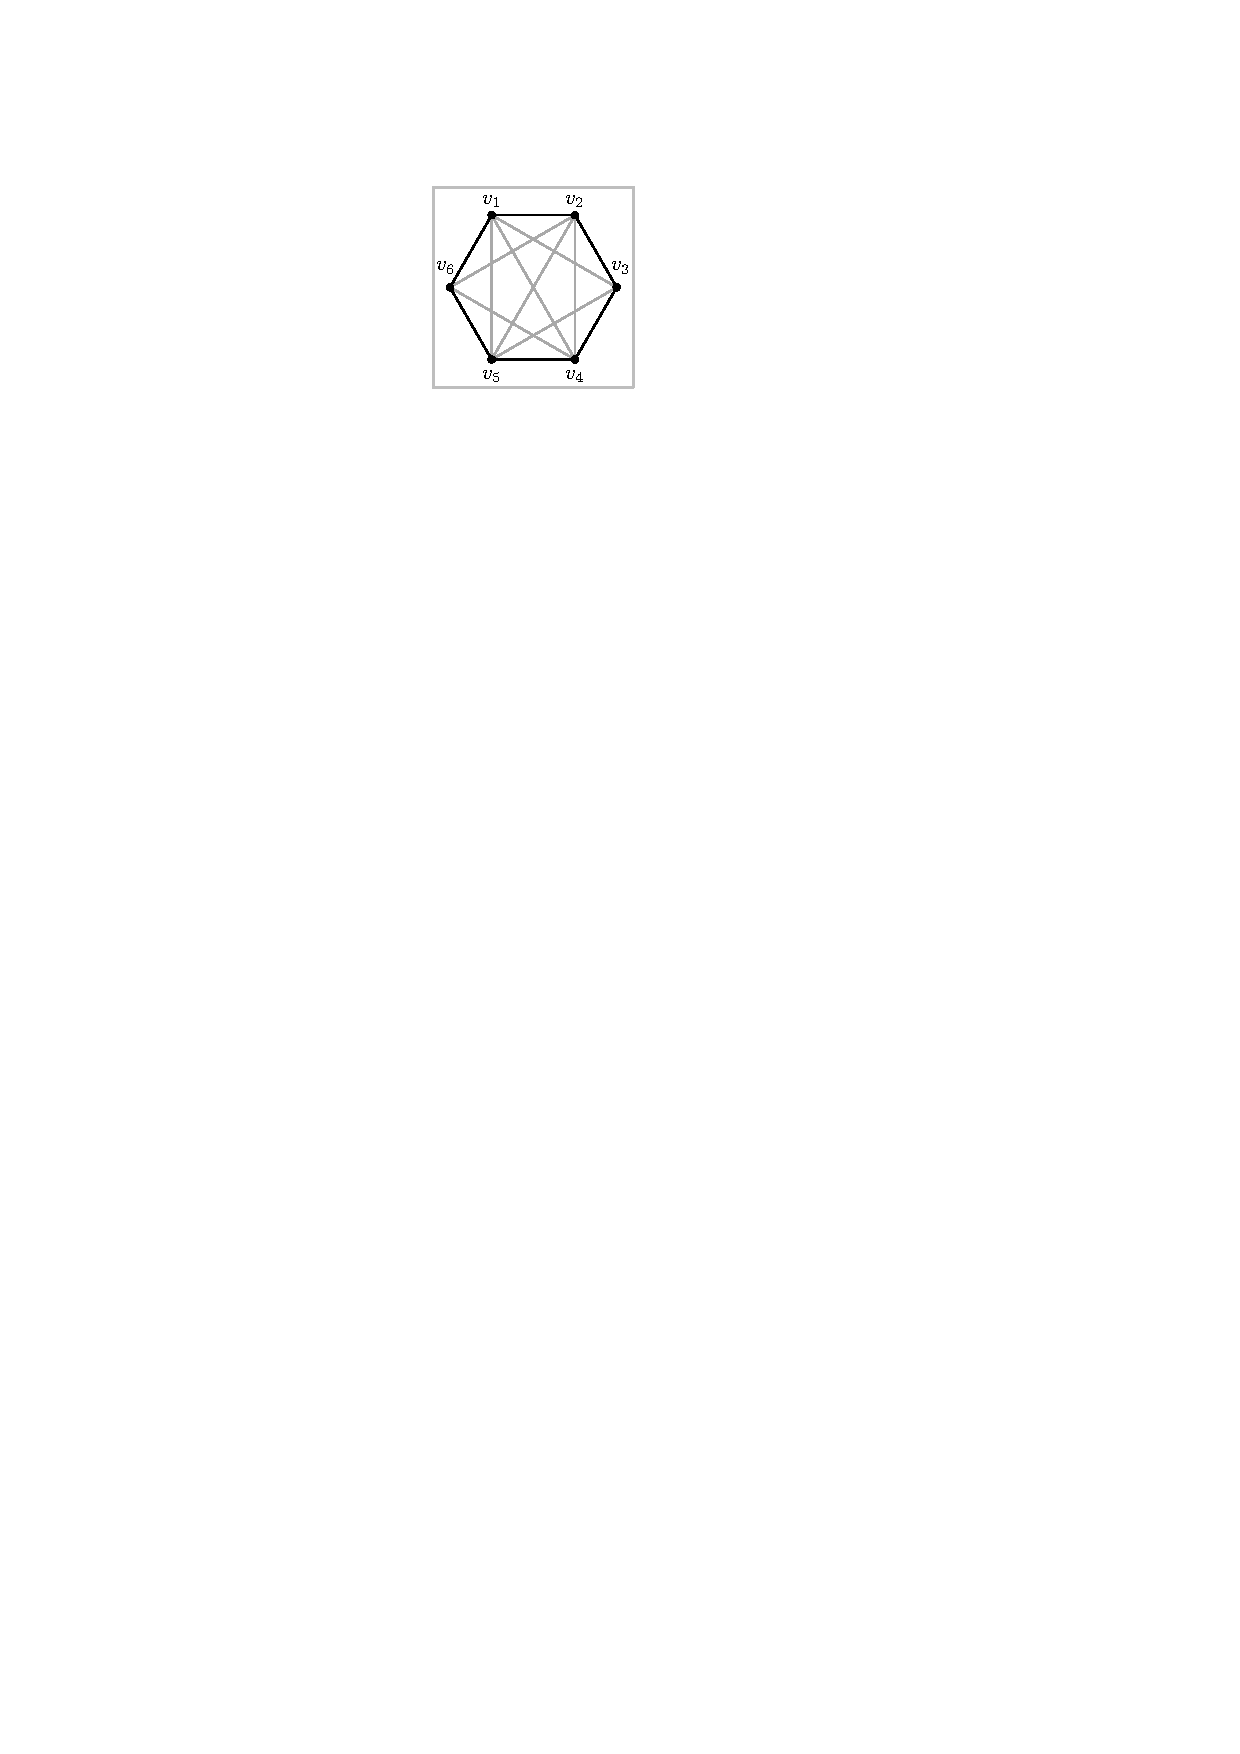
\includegraphics[width=\textwidth,page=1]{images/polygon_conf}
        \subcaption{~}\label{fig:3_planar_polygon_conf_6}
    \end{minipage}
    \begin{minipage}[b]{.24\textwidth}
        \centering
        \includegraphics[width=\textwidth,page=2]{images/polygon_conf}
        \subcaption{~}\label{fig:3_planar_polygon_conf_7}
    \end{minipage}
    \begin{minipage}[b]{.24\textwidth}
        \centering
        \includegraphics[width=\textwidth,page=3]{images/polygon_conf}
        \subcaption{~}\label{fig:3_planar_polygon_conf_8}
    \end{minipage}
    \begin{minipage}[b]{.24\textwidth}
        \centering
        \includegraphics[width=\textwidth,page=4]{images/polygon_conf}
        \subcaption{~}\label{fig:3_planar_polygon_conf_9}
    \end{minipage}
    \begin{minipage}[b]{.24\textwidth}
        \centering
        \includegraphics[width=\textwidth,page=5]{images/polygon_conf}
        \subcaption{~}\label{fig:3_planar_polygon_conf_10}
    \end{minipage}
		\begin{minipage}[b]{.24\textwidth}
        \centering
        \includegraphics[width=\textwidth,page=6]{images/polygon_conf}
        \subcaption{~}\label{fig:3_planar_polygon_conf_7_stick}
    \end{minipage}
    \begin{minipage}[b]{.24\textwidth}
        \centering
        \includegraphics[width=\textwidth,page=7]{images/polygon_conf}
        \subcaption{~}\label{fig:3_planar_polygon_conf_8_stick}
    \end{minipage}
    \caption{%
    Configurations of Lemma~\ref{lem:3_planar_true_planar}.
    \label{fig:3_planar_polygon_conf}}
\end{figure}

Denote by $m_P(k)$ be the maximum number of chords in a true planar $k$-cycle (without vertices in its interior) of the drawing $\Gamma(G)$ as given by Lemma~\ref{lem:3_planar_true_planar}, for $6\leq k\leq 10$. 

\begin{lemma}\label{lem:3_planar_polygon}
Let $\Gamma(G)$ be a PMCM $3$-planar drawing of an optimal $3$-planar graph $G$ on $n$ vertices, and let $k$ such that $6\leq k\leq 9$. Suppose that there exists a \pp $\mathcal{P}_k$ of $k$ vertices in $\Gamma(G)$, such that the boundary edges of $\mathcal{P}_k$ exist in the drawing. Let $E_k$ be the set of edge-segments that pass through $\mathcal{R}_k$, and $m_k=|E_k|$.If: 
\begin{enumerate}
\item $m_k\leq 2k-4$, and, 
\item every edge-segment of $E_k$ has at least one crossing in $\mathcal{R}_k$,
\end{enumerate}
%\todo{replace every edge with every part of any edge}
then there exists a true planar $k'$-cycle in $\Gamma(G)$ (without vertices in its interior), with $k\leq k'\leq 9$, with all edge-segments of $E_k$ as chords.
\end{lemma}

\begin{proof}
Before proving the lemma we need to make the following remark: \todo{perhaps rephrase if not clear}If an edge-segment of an edge $e$ belongs to $E_k$ then no other edge-segment of $e$ lies inside $\mathcal{R}_k$. This is true, since if at least two edge-segments of $e$ lie inside $\mathcal{R}_k$, then each edge-segment has at least one crossing in $\mathcal{R}_k$ (by the assumptions of the lemma) and at least one crossing with the boundary of $\mathcal{P}_k$ (otherwise there would be only one edge-segment of $e$ in $E_k$). Hence, $e$ has at least $4$ crossings in $\Gamma(G)$ which is not allowed. 
 
First, we prove the lemma for the case $k=9$. Let $C$ be the $9$-cycle defined by the boundary of the \pp $\mathcal{P}$, with vertices $v_1,v_2,\dots,v_9$, and let $E$ the set of edge-segments that pass through its \pr $\mathcal{R}$ and apply to the conditions of the lemma. If no edge with edge-segment in $E$ crosses an edge of $C$,  then $C$ is clearly a true planar $9$-cycle, and the lemma holds for $k'=k$. So, suppose that at least one edge with edge-segment in $E$, say $e$ crosses an edge of $C$ (refer to Figure~\ref{fig:3_planar_polygon_before}). W.l.o.g. we can assume that $e$ crosses edge $(v_1,v_2)$ of $C$. Let $c$ be the crossing point of $e$ and $(v_1,v_2)$. If $w$ and $w'$ are the two endpoints of $e$, we have that either edge-segment $(w,c)$ of $e$ or edge-segment $(c,w')$ of $e$ is entirely drawn outside $\mathcal{R}$ (otherwise $e$ would have at least two edge-segments in $E$, which is not possible as explained earlier). Assume w.l.o.g. that  $(w,c)$ part of $e$ is drawn outside $\mathcal{R}$. Then \pes $[v_1,w]$ and $[w,v_2]$ are corner edges. Note that $e$ has already at least two crossings: one in $\mathcal{R}$ (assumption of the lemma) and one with edge $(v_1,v_2)$. This implies that there exists at most one edge, say $e'$ (where $e'$ might have an edge-segment in $E$ or not), crossing with $e$. Vertices $v_1,w,v_2,\dots,v_9$ define a \pp $\mathcal{P}'$ on $10$ vertices (see Figure~\ref{fig:3_planar_polygon_after}) and, for the set of edge-segments $E'$ that pass through its \pr $\mathcal{R}'$, we have that $E'$ contains all edge-segments of $E$ plus at most two more: the open edge-segment defined by $(v_1,v_2)$, and possibly an edge-segment of $e'$. Hence $E'$ defines at most  $16$ edges. However, by Lemma~\ref{lem:3_planar_true_planar}, we can replace $E'$ with a $3$-planar pattern that defines $17$ edges (refer to Figure~\ref{fig:3_planar_polygon_conf_10}). The derived graph has more edges that $G$, a contradiction to the optimality of $G$. Hence we have concluded that for $k=9$, $C$ is a true planar cycle on $9$ vertices.

%First, we prove the lemma for the case $k=9$. Let $C$ be the $9$-cycle defined by the boundary of the \pp $\mathcal{P}$, with vertices $v_1,v_2,\dots,v_9$, and let $E$ the set of edge-segments that pass through its polygonal region $\mathcal{R}$ and apply to the conditions of the lemma. If no edge of $E$ crosses an edge of $C$,  then $C$ is clearly a true planar $9$-cycle, and the lemma holds for $k'=k$. So, suppose that at least one edge, say $e$ crosses an edge of $C$ (refer to Figure~\ref{fig:3_planar_polygon_before}). W.l.o.g. we can assume that $e$ crosses edge $(v_1,v_2)$ of $C$. Let $c$ be the crossing point of $e$ and $(v_1,v_2)$. If $w$ and $w'$ are the two endpoints of $e$, we have that either $(w,c)$ part of $e$ or $(c,w')$ part of $e$ is entirely drawn outside $\mathcal{R}$ (refer to above remark). Assume w.l.o.g. that  $(w,c)$ part of $e$ is drawn outside $\mathcal{R}$. Then edges $(v_1,w)$ and $(w,v_2)$ are potential corner edges. Note that $e$ has already at least two crossings: one in $\mathcal{R}$ (assumption of the lemma) and one with edge $(v_1,v_2)$. This implies that there exists at most one edge, say $e'$, where $e'\notin E$, crossing with $e$. Vertices $v_1,w,v_2,\dots,v_9$ define a \pp $\mathcal{P}'$ on $10$ vertices (see Figure~\ref{fig:3_planar_polygon_after}) and, for the set of edges $E'$ that pass through its polygonal region $\mathcal{R}'$, we have that $E'=E\cup\left\{(v_1,v_2), e'\right\}$, and $|E'|\leq 16$. However, by Lemma~\ref{lem:3_planar_true_planar}, we can replace $E'$ with a $3$-planar pattern that has $17$ edges (refer to Figure~\ref{fig:3_planar_polygon_conf_10}). The derived graph has more edges that $G$, a contradiction to the optimality of $G$. Hence we have concluded that for $k=9$, $C$ is a true planar cycle on $9$ vertices.

Now, for the rest of the cases, assume that the lemma holds for $6<k\leq 9$. We will prove that it also holds for $k-1$. So, let $C$ be a $k-1$-cycle defined by the boundary of a \pp $\mathcal{P}$, with vertices $v_1,v_2,\dots,v_{k-1}$, and let $E$ the set of edge-segments that pass through its \pr $\mathcal{R}$ and apply to the conditions of the lemma. As in the previous case, if no edge with edge-segment in $E$ crosses an edge of $C$,  then $C$ is clearly a true planar $k-1$-cycle, and the lemma holds for $k'=k-1$. So, suppose that at least one edge with edge-segment in $E$, say $e$ crosses an edge of $C$. W.l.o.g. we can assume that $e$ crosses edge $(v_1,v_2)$ of $C$. Let $c$ be the crossing point of $e$ and $(v_1,v_2)$. If $w$ and $w'$ are the two endpoints of $e$, we have that either edge-segment $(w,c)$ of $e$ or edge-segment $(c,w')$ of $e$ is entirely drawn outside $\mathcal{R}$. Assume w.l.o.g. that edge-segment $(w,c)$ of $e$ is drawn outside $\mathcal{R}$. Then \pes $[v_1,w]$ and $[w,v_2]$ are corner edges. Note that $e$ has already at least two crossings: one in $\mathcal{R}$ (assumption of the lemma) and one with edge $(v_1,v_2)$. This implies that there exists at most one edge, say $e'$ (where $e'$ might have an edge-segment in $E$ or not), crossing with $e$. Vertices $v_1,w,v_2,\dots,v_{k-1}$ define a \pp $\mathcal{P}'$ on $k$ vertices and, for the set of edge-segments $E'$ that pass through its polygonal region $\mathcal{R}'$, we have that contains all edge-segments of $E$ plus at most two more: the open edge-segment defined by $(v_1,v_2)$, and possibly an edge-segment of $e'$. Hence $|E'|\leq 2k-4$. However, by Lemma~\ref{lem:3_planar_true_planar}, we can replace $E'$ with a $3$-planar pattern that has $2k-4$ edges (refer to Figures~\ref{fig:3_planar_polygon_conf_7_stick}, \ref{fig:3_planar_polygon_conf_8_stick}, \ref{fig:3_planar_polygon_conf_9} for $k=7,8,9$ resp.). Since $G$ is optimal, the derived graph has the same number of edges as $G$. This can only be true if all boundary edges of $\mathcal{P}'$ exist in $\Gamma(G)$. Then, the vertices of $\mathcal{P}'$ define a $k$-cycle in $\Gamma(G)$ that satisfies the assumptions of the lemma: $|E'|=2k-4$ and every edge-segment of $E'$ has at least one crossing in $\mathcal{R}'$ (this is true for all edge-segments of $E\subset E'$ and also for the edge-segments of $(v_1,v_2)$ and $e'$ since they cross $e$ in the interior of $\mathcal{R}'$). By the induction hypothesis, there exists a true planar cycle on $k'$ vertices, where $k\leq k'\leq 9$, with all edge-segments of $E'$, and therefore of $E$,  as chords.


%Now, for the rest of the cases, assume that the lemma holds for $6<k\leq 9$. We will prove that it also holds for $k-1$. So, let $C$ be a $k-1$-cycle defined by the boundary of a \pp $\mathcal{P}$, with vertices $v_1,v_2,\dots,v_{k-1}$, and let $E$ the set of edge-segments that pass through its polygonal region $\mathcal{R}$\todo{and apply to the conditions of the lemma}. As in the previous case, if no edge of $E$ crosses an edge of $C$,  then $C$ is clearly a true planar $k-1$-cycle, and the lemma holds for $k'=k$. So, suppose that at least one edge, say $e$ crosses an edge of $C$. W.l.o.g. we can assume that $e$ crosses edge $(v_1,v_2)$ of $C$. Let $c$ be the crossing point of $e$ and $(v_1,v_2)$. If $w$ and $w'$ are the two endpoints of $e$, we have that either $(w,c)$ part of $e$ or $(c,w')$ part of $e$ is entirely drawn outside $\mathcal{R}$. Assume w.l.o.g. that  $(w,c)$ part of $e$ is drawn outside $\mathcal{R}$. Then edges $(v_1,w)$ and $(w,v_2)$ are potential corner edges. Note that $e$ has already at least two crossings: one in $\mathcal{R}$ (assumption of the lemma) and one with edge $(v_1,v_2)$. This implies that there exists at most one edge, say $e'$, where $e'\notin E$, crossing with $e$. Vertices $v_1,w,v_2,\dots,v_{k-1}$ define a \pp $\mathcal{P}'$ on $k$ vertices and, for the set of edges $E'$ that pass through its polygonal region $\mathcal{R}'$, we have that $E'=E\cup\left\{(v_1,v_2), e'\right\}$, and $|E'|\leq 2k-4$. However, by Lemma~\ref{lem:3_planar_true_planar}, we can replace $E'$ with a $3$-planar pattern that has $2k-4$ edges (refer to Figures~\ref{fig:3_planar_polygon_conf_7_stick}, \ref{fig:3_planar_polygon_conf_8_stick}, \ref{fig:3_planar_polygon_conf_9} for $k=7,8,9$ resp.). Since $G$ is optimal, the derived graph has the same number of edges as $G$. This can only be true if all boundary edges of $\mathcal{P}'$ exist in $\Gamma(G)$. Then, the vertices of $\mathcal{P}'$ define a $k$-cycle in $\Gamma(G)$ that satisfies the assumptions of the lemma: $|E'|=2k-4$ and every edge\todo{every part of any edge } of $E'$ has at least one crossing in $\mathcal{R}'$ (this is true for all edges of $E\subset E'$ and also for edges $(v_1,v_2)$ and $e'$ since their crossing point $c$ is in the interior of $\mathcal{R}'$). Then there exists a true planar cycle on $k\leq k'\leq 9$ vertices with all edges of $E'$, and therefore of $E$,  as chords.\qed
\end{proof}

%\todo[inline]{move the definition}
Suppose that in a PMCM drawing $\Gamma(G)$ an edge $e$ is crossed by two edges $e_1$ and $e_2$, where $e_i=(u_i,v_i)$ for $i=1,2$. Recall that if $\Gamma(G)$ is almost-simple then at least one of parallel edges $[u_1,u_2]$ and $[v_1,v_2]$ is a \pe of $\Gamma(G)$. Also, in the case where both parallel edges $[u_1,u_2]$ and $[v_1,v_2]$ are \pes of $\Gamma(G)$, $e_1$ and $e_2$ are called independent.

\begin{lemma}\label{lem:3_planar_independent}
Let $\Gamma(G)$ be an almost-simple PMCM $3$-planar drawing of an optimal $3$-planar graph $G$ on $n$ vertices. If an edge is crossed by two independent edges, then it is a chord of a true planar $k$-cycle (without vertices in its interior), with $6\leq k\leq 9$.
\end{lemma}
\begin{proof}
Let $e=(u,v)$ be an edge of $\Gamma(G)$ that crosses with  $e_1$ and $e_2$, where $e_i=(u_i,v_i)$ for $i=1,2$. Since $e_1$ and $e_2$ are independent edges, both parallel edges $[u_1,u_2]$ and $[v_1,v_2]$ are \pes, as in Figure~\ref{fig:3_planar_independent}. Then vertices $u,u_1,u_2,v,v_2,v_1$ define a \pp $\mathcal{P}_6$ of six vertices (grey shaded in Figure~\ref{fig:3_planar_independent}). The \pr $\mathcal{R}_6$ of $\mathcal{P}_6$ contains no vertices in its interior, and at most $8$ edges of $\Gamma(G)$ define edge-segments that pass through $\mathcal{R}_6$: edges $(u,v)$, $(u_1,v_1)$, $(u_2,v_2)$, at most one other edge that crosses $(u,v)$, and at most four other edges that cross $(u_1,v_1)$ or $(u_2,v_2)$. We proceed by removing  edges $(u,v)$, $(u_1,v_1)$, $(u_2,v_2)$ and all other edges that cross $(u,v)$, $(u_1,v_1)$ or $(u_2,v_2)$, and replace them with the $3$-planar pattern of Figure~\ref{fig:3_planar_polygon_conf_6}. In the derived graph there exist $8$ edges drawn in $\mathcal{R}_6$ and do not cross the boundary of the \pp. Since $G$ is optimal, all boundary edges of $\mathcal{P}_6$ already exist in $\Gamma(G)$. Furthermore, all edge-segments that pass through $\mathcal{R}_6$ have at least one crossing in $\mathcal{R}_6$. Then, we can apply Lemma~\ref{lem:3_planar_polygon}, and conclude that there exists a true planar $k$-cycle without vertices in its interior ($6\leq k\leq 9$), that contains $e$ as a chord.
\end{proof}

%\begin{lemma}\label{lem:3_planar_independent}
%Let $\Gamma(G)$ be a $3$-planar drawing of an optimal $3$-planar graph $G$ on $n$ vertices. If an edge is crossed by two independent parallel edges, then it is a chord of a true planar $k$-cycle (without vertices in its interior), with $6\leq k\leq 9$.
%\end{lemma}
%\begin{proof}
%Let $e=(u,v)$ be an edge of $\Gamma(G)$ that crosses with  $e_1$ and $e_2$, where $e_i=(u_i,v_i)$ for $i=1,2$. Since $e_1$ and $e_2$ are independent parallel edges, both potential parallel edges $(u_1,u_2)$ and $(v_1,v_2)$ exist, as in Figure~\ref{fig:3_planar_independent}. Then vertices $u,u_1,u_2,v,v_2,v_1$ define a \pp $\mathcal{P}_6$ of six vertices (grey shaded in Figure~\ref{fig:3_planar_independent}). The polygonal region $\mathcal{R}_6$ of $\mathcal{P}_6$ contains no vertices in its interior, and at most $8$ edges of $\Gamma(G)$ pass through $\mathcal{R}_6$: edges $(u,v)$, $(u_1,v_1)$, $(u_2,v_2)$, at most one other edge that crosses $(u,v)$, and at most four other edges that cross $(u_1,v_1)$ or $(u_2,v_2)$. We proceed by removing  edges $(u,v)$, $(u_1,v_1)$, $(u_2,v_2)$ and all other edges that cross $(u,v)$, $(u_1,v_1)$ or $(u_2,v_2)$, and replace them with the $3$-planar pattern of Figure~\ref{fig:3_planar_polygon_conf_6}. In the derived graph there exist $8$ edges drawn in $\mathcal{R}_6$ and do not cross the boundary of the \pp. Since $G$ is optimal, all boundary edges of $\mathcal{P}_6$ already exist in $\Gamma(G)$. Then, we can apply Lemma~\ref{lem:3_planar_polygon}, and conclude that there exists a true planar $k$-cycle without vertices in its interior ($6\leq k\leq 9$), that contains $e$ as a chord.\qed
%\end{proof}

\begin{figure}[htb]
    \centering
    \begin{minipage}[b]{.24\textwidth}
        \centering
        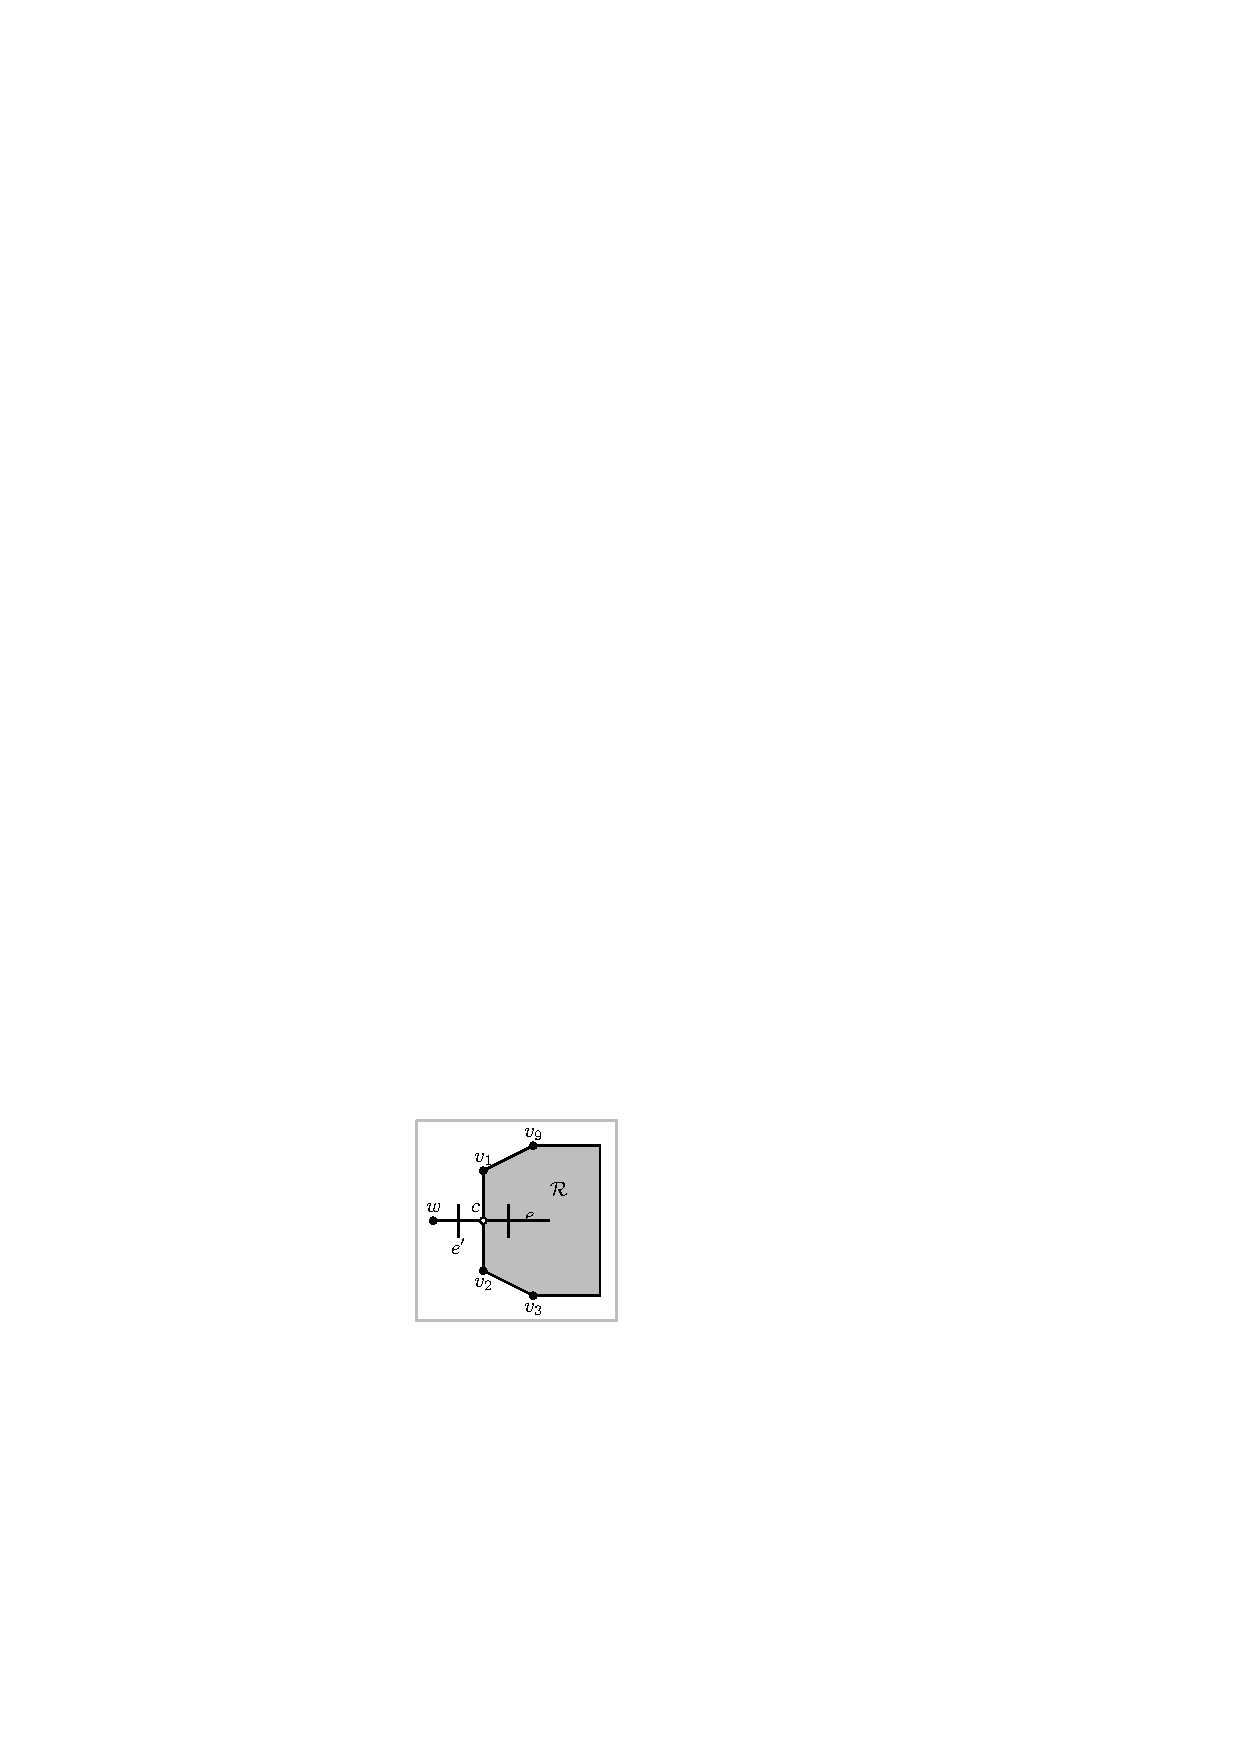
\includegraphics[width=\textwidth,page=1]{images/3planar_polygon}
        \subcaption{~}\label{fig:3_planar_polygon_before}
    \end{minipage}
    \begin{minipage}[b]{.24\textwidth}
        \centering
        \includegraphics[width=\textwidth,page=2]{images/3planar_polygon}
        \subcaption{~}\label{fig:3_planar_polygon_after}
    \end{minipage}
    \begin{minipage}[b]{.24\textwidth}
        \centering
        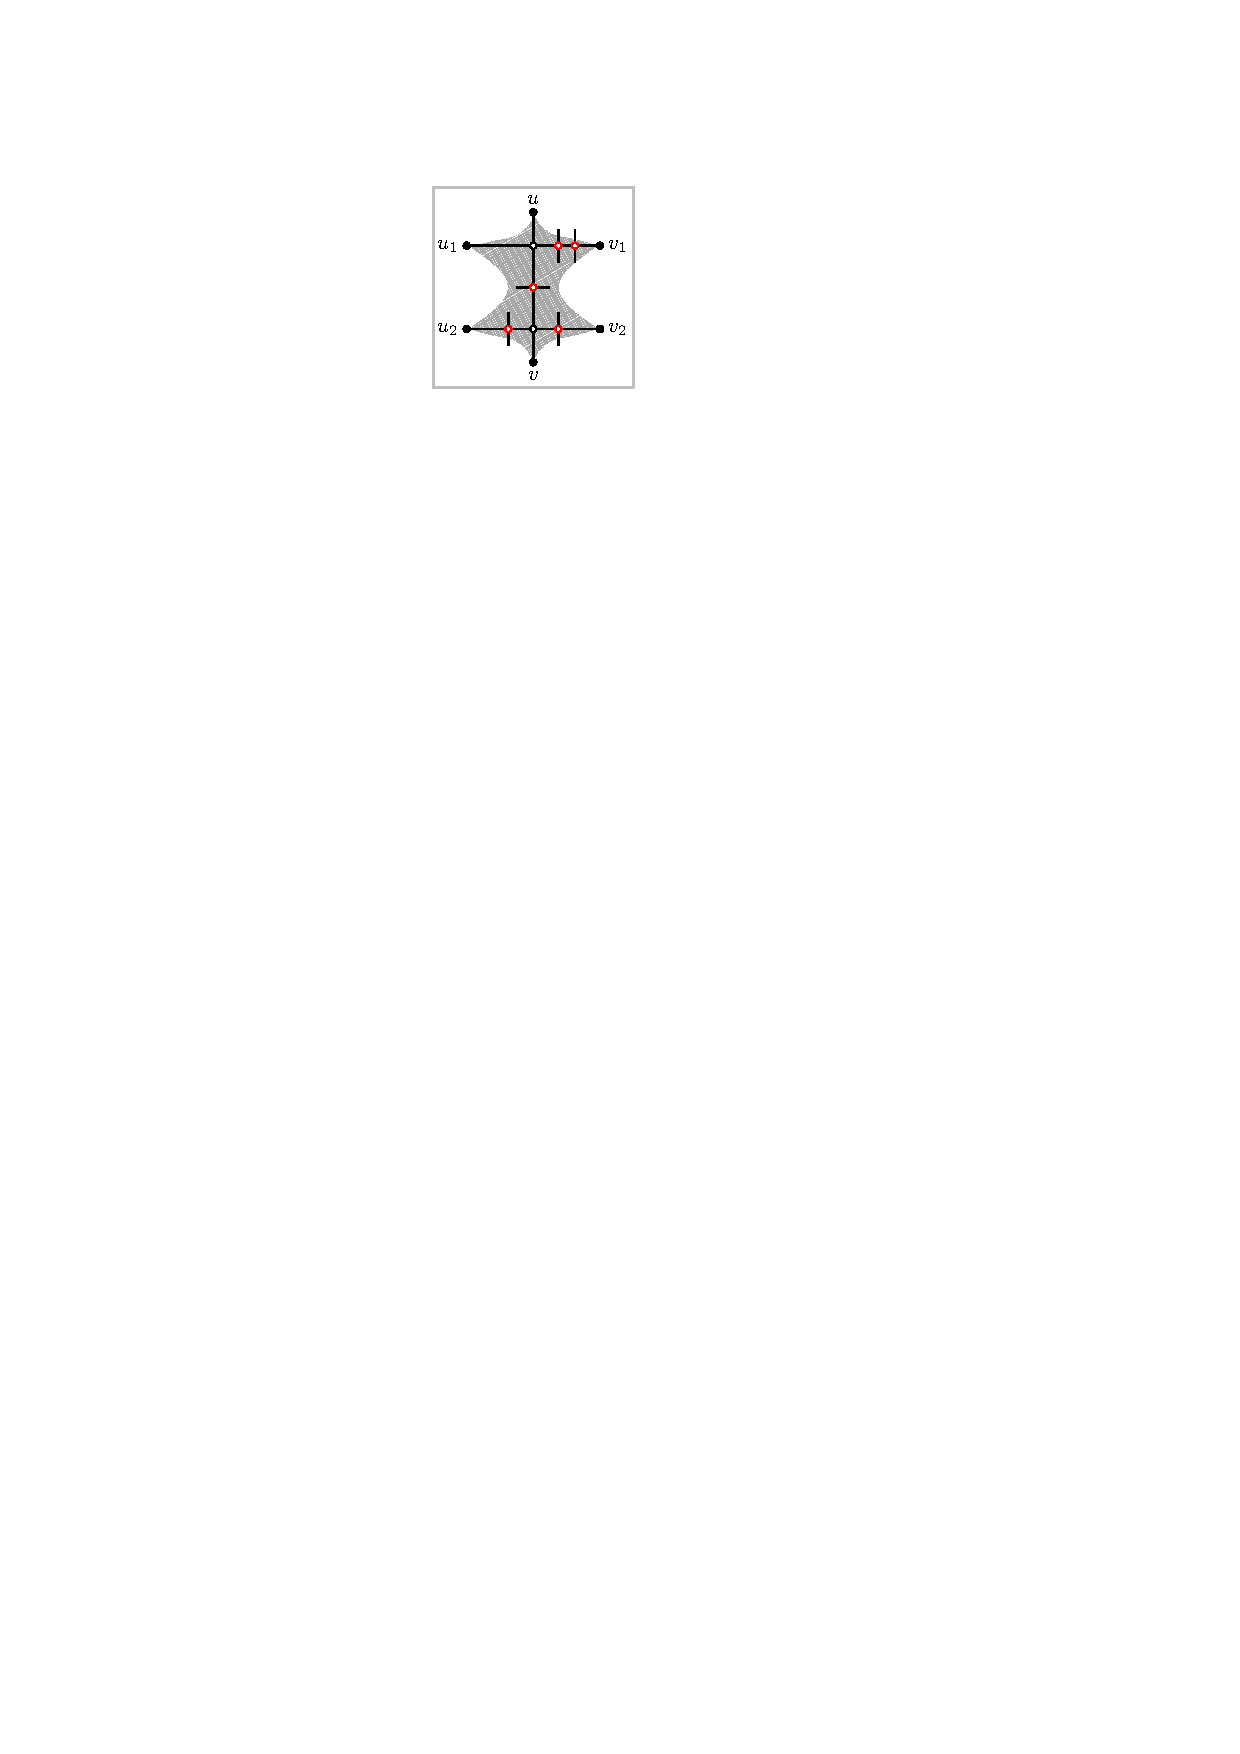
\includegraphics[width=\textwidth,page=1]{images/3planar_independent}
        \subcaption{~}\label{fig:3_planar_independent}
    \end{minipage}
    \caption{%
    (a)-(b):~Configurations of Lemma~\ref{lem:3_planar_polygon}, (c):~Configuration of Lemma~\ref{lem:3_planar_independent}}.
    \label{fig:3_planar_polygon}
\end{figure}


\todo[inline]{move the definition}
Consider the so called crossing graph $G_C$ of the drawing $\Gamma(G)$. The vertices of $G_C$ correspond to the edges of $G$ and two vertices of $G_C$ are adjacent if and only if the corresponding edges of $G$ cross in $\Gamma(G)$. The connected components of $G_C$ define a partition of the edges $E(G)$ of $G$ to \emph{propagated sets of crossing edges}. If $e\in E(G)$ we denote by $S(e)$ the unique propagated set of crossing edges that $e$ belongs to. Note that if $e$ is a chord of a true planar $k$-cycle in the drawing $\Gamma(G)$ that has no vertices in its interior, then all edges of $S(e)$ are also chords of the $k$-cycle.

Now we are ready to state the main property of almost-simple PMCM-drawings of optimal $3$-planar  graphs:

\begin{lemma}\label{lem:3_planar_small_faces}
Let $\Gamma(G)$ be an almost-simple PMCM $3$-planar drawing of an optimal $3$-planar graph $G$ on $n$ vertices. Any edge that is crossed three times in  $\Gamma(G)$ is a chord of a true-planar $k$-cycle in $\Gamma(G)$ (without vertices in its interior), where $6\leq k\leq 9$. 
\end{lemma}

\begin{proof}
Let $e=(u,v)$ be an edge of $G$ that crosses with edges $e_i=(u_i,v_i)$ in $\Gamma(G)$, for $i=1,2,3$. Consider the propagated set of crossing edges $S(e)$ where $e$ belongs to. We distinguish two cases depending on whether there exists an edge in $S(e)$ that crosses with two independent edges or not.

Suppose that this is the case, and an edge of $S(e)$ is crossed by two independent edges. Then by Lemma~\ref{lem:3_planar_independent}, there exists a true planar $k$-cycle (without vertices in its interior) defining a \pr with this edge as a chord. Then all edges of $S(e)$ are also drawn as chords of the $k$-cycle and the lemma follows.

Assume, now that all edges of $S(e)$ with at least two crossings, are not crossed by independent edges in $\Gamma(G)$. Then, for edge $e$, that crosses with edges $e_1$, $e_2$, and $e_3$, we have that edges $e_i$, $e_j$ ($1\leq i<j\leq 3$) are not parallel edges. This implies that exactly one of parallel edges $[u_i,u_j]$ or $[v_i,v_j]$ is not a \pe. For the sake of simplicity let's refer to parallel edges $[u_i,u_j]$ and $[v_i,v_j]$ as the ``$u$-parallel edge'' and ``$v$-parallel edge'' respectively of $e_i$ and $e_j$. 
There are three ways to combine indices $i$ and $j$ and for every combination exactly one of the ``$u$-parallel edge'' and ``$v$-parallel edge'' is not a \pe. This implies that: there exist at least two combinations such that their ``$u$-parallel edges'' are not \pes, or there exist at least two combinations such that their ``$v$-parallel edges'' are not \pes of $\Gamma(G)$. W.l.o.g. assume that there exist two combinations of indices, say $i_1$ with $j_1$ and $i_2$ with $j_2$ for which their ``$u$-parallel edges'', namely $[u_{i_1},u_{j_1}]$ and $[u_{i_2},u_{j_2}]$  are not \pes. It is clear that since $i_1\neq j_1$, $i_2\neq j_2$ and $\left\{i_1,i_2,j_1,j_2\right\}\subset\left\{1,2,3\right\}$, at least two indices are the same. W.l.o.g. assume that $i_1=i_2$; other cases are symmetric. Let$i=i_1=i_2$. Then we have that parallel edges  $(u_i,u_{j_1})$ and $(u_i,u_{j_2})$ are not \pes, where $j_1\neq j_2$. This implies that $u_i=u_{j_1}$ and $u_i=u_{j_2}$. It is not hard to see that parallel edge $(u_{j_1},u_{j_2})$ can not be a \pe either; for an example refer to Figure~\ref{fig:3_planar_small_faces_example}, where $i=1$. Hence, for any edge of $S(e)$ with three crossings in $\Gamma(G)$, we have the crossing pattern of Figure~\ref{fig:3_planar_small_faces_conf}, where the grey-shaded region has no vertices in its interior.

%Since there are three pairs of potential parallel edges $e_i$ and $e_j$, there exist at least two pairs, say $e_i$-$e_j$ and $e_{i'}$-$e_{j'}$ for which both \pes $(u_i,u_j)$ and $(u_{i'},u_{j'})$, or both \pes $(v_i,v_j)$ and $(v_{i'},v_{j'})$ do not exist. Assume w.l.o.g. that edges $(u_i,u_j)$ and $(u_{i'},u_{j'})$ do not exist. Since $1\leq i,i',j,j'\leq 3$ and $i\neq j$, $i'\neq j'$, we can also assume that $i=i'$. Then we have that potential parallel edges  $(u_i,u_j)$ and $(u_i,u_{j'})$ do not exist. This implies that $u_i=u_j$ and $u_i=u_j'$. Also, the potential parallel edge $(u_j,u_{j'})$ can not exist, since otherwise at least one of potential parallel edges $(u_i,u_j)$ or $(u_i,u_{j'})$ would also exist (for an example refer to Figure~\ref{fig:3_planar_small_faces_example}, where $i=1$). Hence, for any edge of $S(e)$ with three crossings in $\Gamma(G)$, we have the crossing pattern of Figure~\ref{fig:3_planar_small_faces_conf}, where the grey-shaded region has no vertices in its interior.

So far, vertices $u,v_1,v_2,v_3,v,u_1$ define a \pp $\mathcal{P}$ on six vertices. We want to apply Lemma~\ref{lem:3_planar_polygon} for $k=6$, and to achieve this, we claim that there exist at most $8$ edges that pass through the \pr $\mathcal{R}$ of $\mathcal{P}$ and satisfy the lemma requirements, and also that all boundary edges of $\mathcal{P}$ exist in $\Gamma(G)$. So, suppose that there exists an edge $e'=(u',v')$ that crosses with $e_2$ in the interior of $\mathcal{R}$. Since $e_2\in S(e)$, $e_2$ is not crossed by independent edges. So, edges $e'=(u',v')$ and $e=(u,v)$ are not independent edges, and exactly one of parallel edges $[u,u']$ or $[v,v']$ is not a \pe. Assume w.l.o.g. that parallel edge $[u,u']$ is not a \pe. This implies that $u=u'$ and that the region $R$ defined by edges $e_2$, $e$ and $e'$ has no vertices in its interior (see Figure~\ref{fig:3_planar_small_faces_conf_middle_a}). Then, $e'$ must cross with $e_1$, as otherwise vertex $v_1$ would be in the interior of $R$; refer to Figure~\ref{fig:3_planar_small_faces_conf_middle_b}. Hence, any edge that crosses with $e_2$, must also cross with $e_1$ or $e_3$. Then, there exist at most four other edges that pass through the polygonal region $\mathcal{R}$ and cross with edges $e_1$, $e_2$ or $e_3$, i.e. we have at most $8$ edges that pass through $\mathcal{R}$. We proceed by removing edges $e$, $e_i$ and all edges that cross with edges $e_i$ in  $\mathcal{R}$ ($i=1,2,3$), and replace them with the $3$-planar pattern of Figure~\ref{fig:3_planar_polygon_conf_6}. The derived graph has at least as many edges as $G$, and since $G$ is optimal, the boundary edges of $\mathcal{P}$ exist in the drawing $\Gamma(G)$. So, the vertices of $\mathcal{P}$ define a $6$-cycle in $\Gamma(G)$ (without vertices in its interior), with $8=2*6-4$ edge-segments passing through $\mathcal{R}$, and these edge-segments have at least one crossing inside $\mathcal{R}$. By Lemma~\ref{lem:3_planar_polygon}, for $k=6$, we have that $e$ is a chord of a true planar $k'$-cycle for $6\leq k'\leq 9$.
\end{proof}

\begin{figure}[htb]
    \centering
    \begin{minipage}[b]{.24\textwidth}
        \centering
        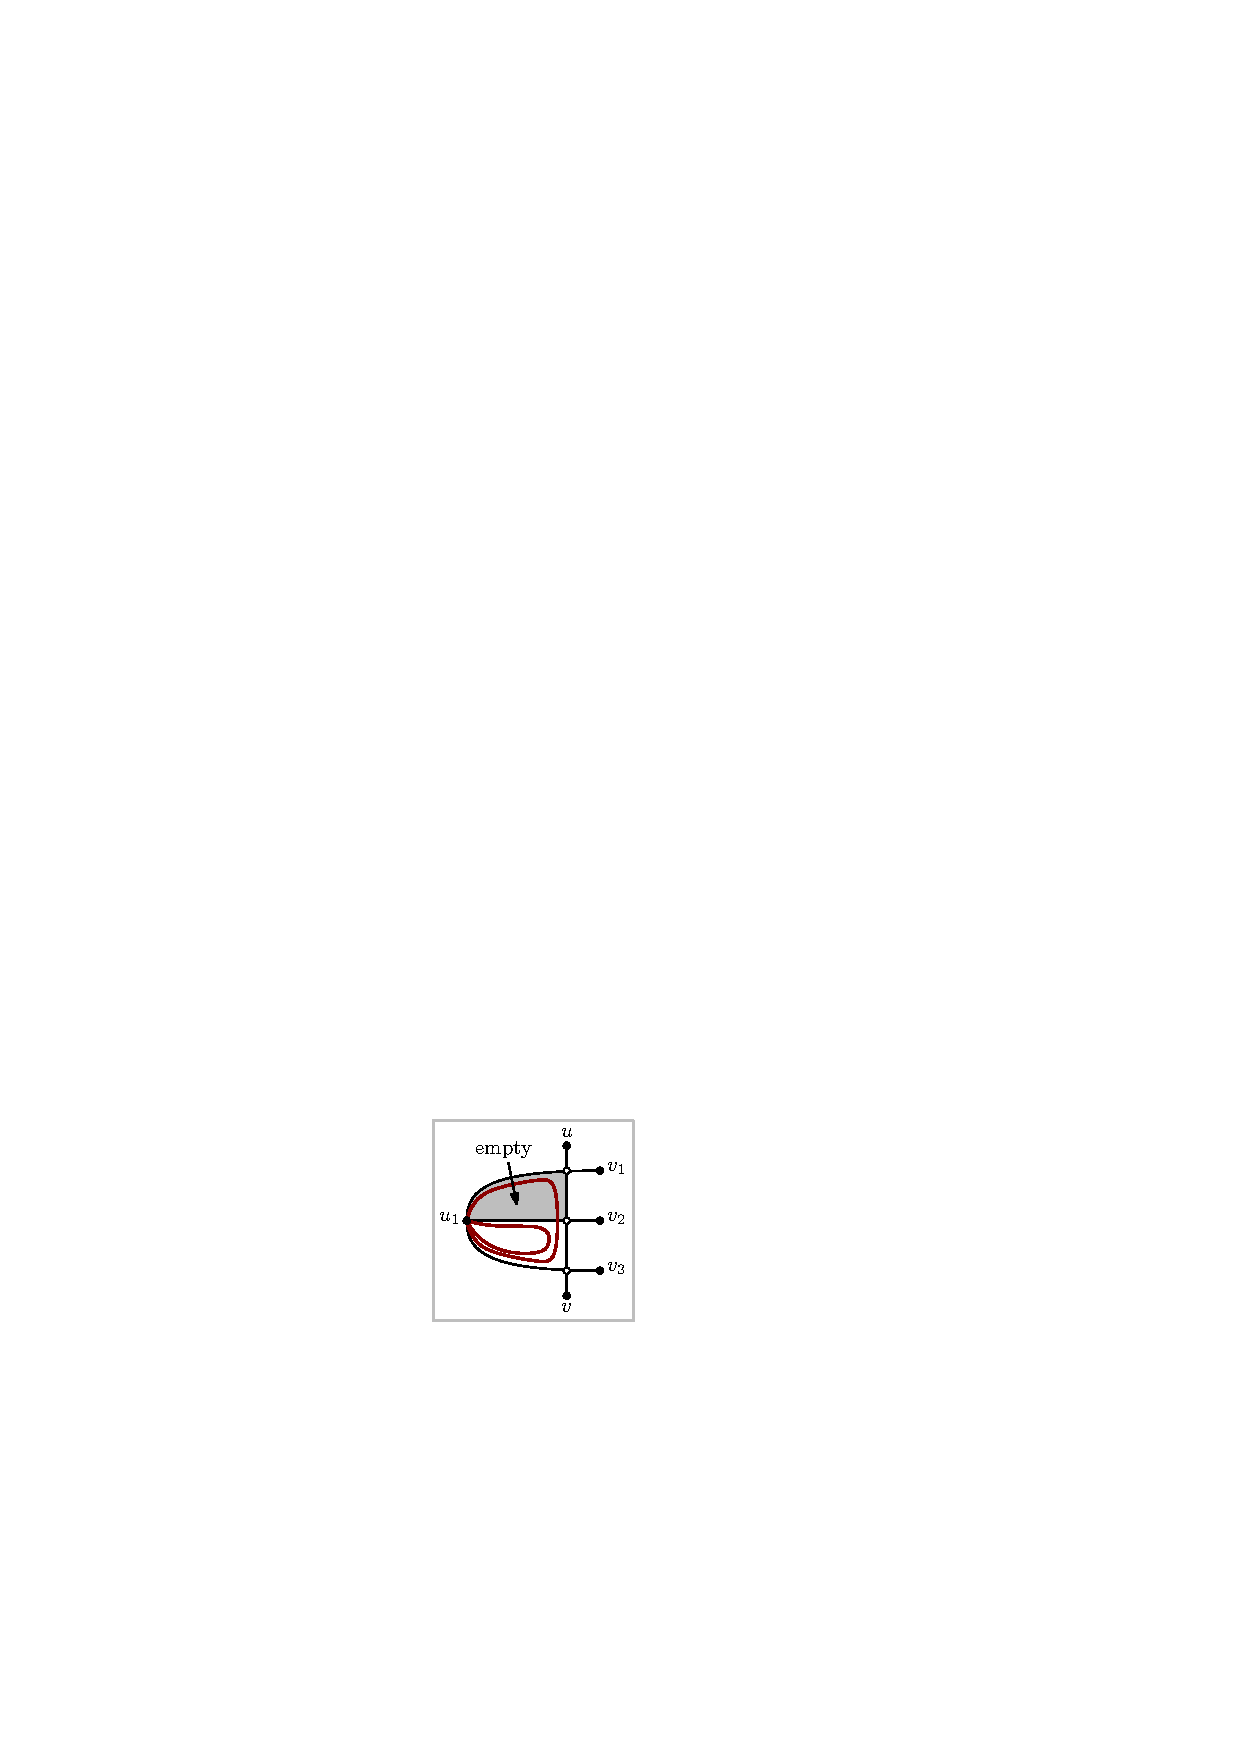
\includegraphics[width=\textwidth,page=1]{images/3planar_small_faces}
        \subcaption{~}\label{fig:3_planar_small_faces_example}
    \end{minipage}
    \begin{minipage}[b]{.24\textwidth}
        \centering
        \includegraphics[width=\textwidth,page=2]{images/3planar_small_faces}
        \subcaption{~}\label{fig:3_planar_small_faces_conf}
    \end{minipage}
    \begin{minipage}[b]{.24\textwidth}
        \centering
        \includegraphics[width=\textwidth,page=3]{images/3planar_small_faces}
        \subcaption{~}\label{fig:3_planar_small_faces_conf_middle_a}
    \end{minipage}
		\begin{minipage}[b]{.24\textwidth}
        \centering
        \includegraphics[width=\textwidth,page=4]{images/3planar_small_faces}
        \subcaption{~}\label{fig:3_planar_small_faces_conf_middle_b}
    \end{minipage}
    \caption{%
    (a):~If the parallel edge $[u_1,u_1]$ is a\pe for edges $(u_2,v_2)$ and $(u_3,v_3)$ then it is also a \pe for edges $(u_1,v_1)$ and $(u_3,v_3)$.  (b)-(d):~Configuration of Lemma~\ref{lem:3_planar_small_faces}.}
    \label{fig:3_planar_small_faces}
\end{figure}

By Lemma~\ref{lem:3_planar_small_faces}, we have that any edge of $G$ that is crossed three times in $\Gamma(G)$ is a chord of a true-planar $k$-cycle (without vertices in its interior) for $6\leq k\leq9$. So, it remains to consider edges of $G$ that have at most two crossings in $\Gamma(G)$, i.e. propagated sets of crossing edges where every edge has at most two crossings. Note that we can not use directly  Lemma~\ref{lem:2_planar_small_faces}, since its proof is based on the fact that optimal $2$-planar graphs have at most $5n-10$ edges, however, we can formulate its analogue lemma as follows:
\begin{lemma}
Let $\Gamma(G)$ be an almost-simple PMCM $3$-planar drawing of an optimal $3$-planar graph $G$ on $n$ vertices. Let $S$ be a propagated set of crossing edges where every edge has at most two crossings. Then edges of $S$ are chords of a true-planar $5$-cycle in $\Gamma(G)$, that contains no vertices in its interior. 
\label{lem:3_planar_small_faces_2}
\end{lemma}
\begin{proof}
We distinguish two cases depending on whether $S$ contains an edge with two crossings or not. Suppose first that this is not the case. Then all edges of $S$ have at most one crossing. Let $e\in S$ crossing with $e'\in S$. Clearly $S=\left\{e,e'\right\}$. The four endpoints of edges $e$ and $e'$ define a \pp $\mathcal{P}$ on $4$ vertices, as in Figure~\ref{fig:3_planar_one_crossing_before} and there are no other edges passing through the \pr $\mathcal{R}$ of $\mathcal{P}$. We proceed by removing edges $e$ and $e'$ and replace them with the $3$-planar pattern of Figure~\ref{fig:3_planar_one_crossing_after}. The derived graph $G'$ has $n'=n+1$ vertices and $m'=m-2+8$ edges, where $n$ and $m$ are the number of vertices and edges of $G$ respectively. Then, $G'$ is $3$-planar and has $m'=5.5n'-10.5>5.5n'-11$ edges; a contradiction.

Now, assume that there exists an edge $e\in S$, where $e=(u,v)$ crossing with two edges $e_1=(u_1,v_1)$ and $e_2=(u_2,v_2)$. By Lemma~\ref{lem:3_planar_independent} edges $e_1$ and $e_2$ are not independent edges. Following the proof of Lemma~\ref{lem:2_planar_small_faces} we can find:
\begin{enumerate}
\item  a \pp on five vertices whose boundary edges define a true planar $5$-cycle with $e$ as a chord, or,
\item a \pp $\mathcal{P}$ on six vertices with at most $6$ edges passing through its \pr  $\mathcal{R}$. In this case, we remove all edges that pass through $\mathcal{R}$ and use the $3$-planar pattern of Figure~\ref{fig:3_planar_polygon_conf_6} that gives $8$ edges in $\mathcal{R}$. The derived graph clearly has more edges than $G$, contradicting its optimality.
\end{enumerate}
\qed
\end{proof}

\begin{figure}[htb]
    \centering
    \begin{minipage}[b]{.24\textwidth}
        \centering
        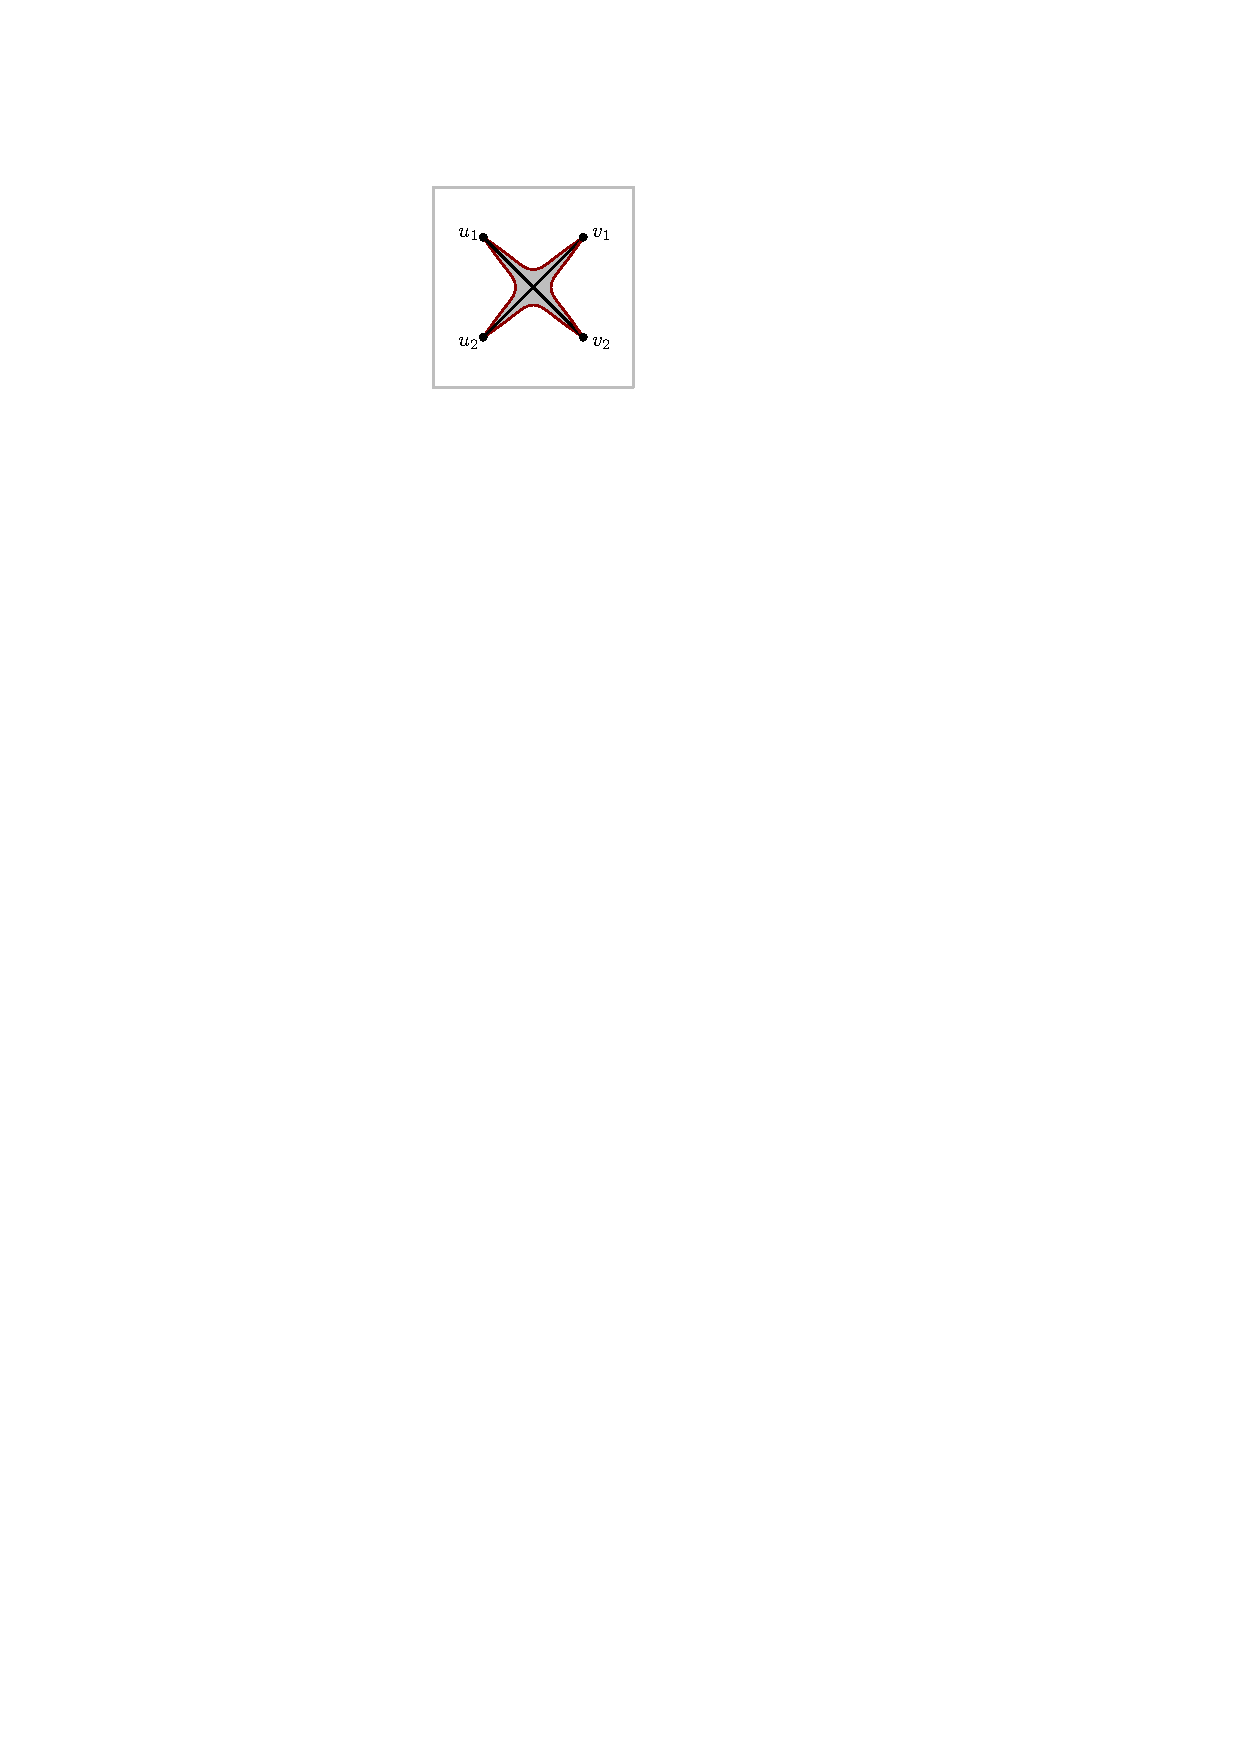
\includegraphics[width=\textwidth,page=1]{images/3planar_one_crossing}
        \subcaption{~}\label{fig:3_planar_one_crossing_before}
    \end{minipage}
    \begin{minipage}[b]{.24\textwidth}
        \centering
        \includegraphics[width=\textwidth,page=2]{images/3planar_one_crossing}
        \subcaption{~}\label{fig:3_planar_one_crossing_after}
    \end{minipage}
		\begin{minipage}[b]{.24\textwidth}
        \centering
        \includegraphics[width=\textwidth,page=3]{images/3planar_one_crossing}
        \subcaption{~}\label{fig:3_planar_triangle}
    \end{minipage}
    \caption{%
    (a)-(b):~Configurations used in Lemma~\ref{lem:3_planar_small_faces_2}. (c):~Configuration used in Lemma~\ref{lem:3_planar_triangle}}.
    \label{fig:3_planar_one_crossing_1}
\end{figure}

\begin{lemma}
Let $\Gamma(G)$ be an almost-simple PMCM $3$-planar drawing of an optimal $3$-planar graph $G$ on $n$ vertices. There is no true planar $3$-cycle without vertices in its interior. 
\label{lem:3_planar_triangle}
\end{lemma}
\begin{proof}
Suppose that there exists a true planar $3$-cycle in $\Gamma(G)$ without vertices in its interior. Then we can add a vertex in the interior of this cycle, and $6$ edges by using the $3$-planar pattern of Figure~\ref{fig:3_planar_triangle}. The derived graph $G'$ has $n'=n+1$ vertices and $m'=m+6$ edges, where $n$ and $m$ are the number of vertices and edges of $G$ respectively. Then, $G'$ is $3$-planar and has $m'=5.5n'-10.5>5.5n'-11$ edges; a contradiction.
\qed
\end{proof}


By combining Lemmas~\ref{lem:3_planar_small_faces}, \ref{lem:3_planar_small_faces_2} and \ref{lem:3_planar_triangle} the following is straightforward:
 
\begin{corollary}\label{cor:3_planar_faces_general}
The true planar structure $\Pi(G)$ of an almost-simple PMCM $3$-planar drawing of an optimal $3$-planar graph $G$ on $n$ vertices contains faces of length at least $5$ and at most $9$.
\end{corollary}

 
 Now we are ready to prove the main property of almost-simple PMCM $3$-planar drawings of optimal $3$-planar graphs.
 
 \begin{lemma}\label{lem:3_planar_faces_final}
  The true planar structure $\Pi(G)$ of an almost-simple PMCM $3$-planar drawing of an optimal $3$-planar graph $G$ on $n$ vertices contains only faces of length $6$.
 \end{lemma}

 \begin{proof}
  Let $e_{TP}$ be the total number of true planar edges of $G$. By Euler's formula we have that
  
  \begin{equation}
   e_{TP}+2=n+f
  \end{equation}
  
  where $f$ is the total number of faces of $G_{TP}$. Let $s_i$ be the number of faces of $G_{TP}$ of length $i$. By Corollary~\ref{cor:3_planar_faces_general} we have that $5\leq i\leq 9$. Hence,
  
  \begin{equation}
   f=s_5+s_6+s_7+s_8+s_9
  \end{equation}

  Also, by counting the edges of all faces of $G_{TP}$ we have that
  
  \begin{equation}
   2e_{T}=5s_5+6s_6+7s_7+8s_8+9s_9
  \end{equation}

  On the other hand for the number of crossing edges of $G$, say $e_{CR}$, by Lemmas~\ref{lem:3_planar_true_planar} and \ref{lem:3_planar_small_faces_2} we have
  
  \begin{equation}
   e_{CR}=5s_5+8s_6+9s_7+11s_8+14s_9
  \end{equation}

  Hence, for the total number of edges of $G$ we have 
	%\todo{rewrite the equations}
  

  $\begin{array}{ll}
   |E(G)|= & 5.5n-11\\
    \Rightarrow &e_{TP}+e_{CR}= 5.5n-11\\
    \Rightarrow &e_{TP}+e_{CR}= 5.5(e_{TP}-f)\\
    \Rightarrow &2e_{CR}= 9e_{TP}-11f\\
    \Rightarrow &10s_5+16s_6+18s_7+22s_8+28s_9 = 4.5(5s_5+6s_6+7s_7+8s_8+9s_9)\\
   &-11(s_5+s_6+s_7+s_8+s_9)\\
    \Rightarrow &10s_5+16s_6+18s_7+22s_8+28s_9=11s_5+16s_6+20.5s_7+25s_829.5s_9\\
    \Rightarrow &0= s_5+2.5s_7+3s_8+1.5s_9\\
   \Rightarrow &0=s_5=s_7=s_8=s_9
  \end{array}$

The last equation implies that there are only faces of length $6$, hence $f=f_6$.
 \end{proof}

Recall that at the beginning of this section we made the assumption that $\Gamma(G)$ is almost-simple, i.e. there is no pair of edges that cross twice in the drawing $\Gamma(G)$. In the following, we prove that in any PMCM drawing of an optimal $3$-planar graph $G$ on $n$ vertices there are no such pairs of edges.
 %By Lemma~\ref{lem:2_planar_faces} we can characterize all maximal $2$-planar graphs. Since the true planar subgraph of such a graph contains only faces of length $5$, we can start with a $5$-tiling of the plane. Now in the interior of every face of length $5$, we can add all  $5$ missing edges.

\begin{lemma}
Let $\Gamma(G)$ be a PMCM $3$-planar drawing of an optimal $3$-planar graph $G$ on $n$ vertices. Then $\Gamma(G)$ is almost-simple.
%There is no pair of edges that cross twice in $\Gamma(G)$. 
\label{lem:3_planar_cross_twice}
\end{lemma}

\begin{proof}
For a proof by contradiction, suppose that there exist edges $(u_1,v_1)$ and $(u_2,v_2)$ that cross twice at crossing points $c_1$ and $c_2$ as in Figure~\ref{fig:3_planar_cross_twice_general}. Consider the bounded region $\mathcal{R}_{IN}$ defined by $(c_1,c_2)$ segment of edges $(u_1,v_1)$ and $(u_2,v_2)$. Let $V_{IN}\subset V(G)$ be the subset of vertices of $G$ that lie in the interior of $\mathcal{R}_{IN}$. By Lemma~\ref{lem:crossing_twice} $|V_{IN}|\geq 1$. Also, since edges $(u_1,v_1)$ and $(u_2,v_2)$ have already two crossings, there exist at most one edge $e'_1$ and an edge $e'_2$ that cross with $(u_1,v_1)$ and $(u_2,v_2)$ respectively. Since $G$ is connected \todo{mention that G is connected} at least one of $e'_1$ or $e'_2$ has an endpoint in $V_{IN}$. Suppose w.l.o.g. that $e'_1$ is an edge incident to vertex $w$, where $w\in V_{IN}$. Note that vertices $u_1$-$u_2$ define a corner pair of vertices and therefore the corner edge $[u_1,u_2]$ is a \pe (refer to the upper red edge of Figure~\ref{fig:3_planar_cross_twice_region}). Also, since $V_{IN}$ is not empty, another \pe $[u_1,u_2]$ exists (refer to the lower red edge of Figure~\ref{fig:3_planar_cross_twice_region}), such that the bounded region defined by these two \pes contains only $V_{IN}$ in its interior. Let $E_w$ be the set of edges of $G$ that have both endpoints in $V_{IN}$ and cross with edge $e'_1$ in the drawing $\Gamma(G)$ (refer to the light red edge of Figure~\ref{fig:3_planar_cross_twice_region}). Denote by $m_w$ the number of edges in $E_w$. Since $e'_1$ already crosses with edge $(u_1,v_1)$, $m_w\leq 2$. Now we distinguish two cases depending on whether $|V_{IN}|=1$ or $|V_{IN}|\geq 2$.

In the first case, we have that $V_{IN}=\left\{w\right\}$ and edge $E_w$ must be empty, i.e. $m_w=0$. We proceed by removing edges $(u_1,v_1)$, $(u_2,v_2)$ and any other edge that crosses with them, and replace them with the $3$-planar pattern of Figure\ref{fig:3_planar_cross_twice_single}. We add a vertex, say $x$ and true planar edges $(u_1,x)$ and $(x,w)$. Vertices $u_1$, $x$, $w$, $x$, $u_1$, $u_2$ define a \pp $\mathcal{P}$ on six vertices (grey shaded in Figure~\ref{fig:3_planar_cross_twice_single}). In the interior of $\mathcal{P}$ we can add $8$ edges by using the $3$-planar pattern of Figure~\ref{fig:3_planar_polygon_conf_6}. The derived graph, say $G'$, has $n'=n+1$ vertices and at least $m'=m-4+10$ edges, where $n$ and $m$ are the number of vertices and edges of $G$ respectively. Hence $G'$ has $m'\geq 5.5n'-10.5>5.5n'-11$, i.e. more edges than allowed, a clear contradiction.

In the second case, where $|V_{IN}|\geq 2$, we proceed by removing edges $(u_1,v_1)$, $(u_2,v_2)$, any other edge that crosses with them, and edges of $E_w$, i.e. we remove at most $4+m_w$ edges. We replace them with the $3$-planar pattern of Figure\ref{fig:3_planar_cross_twice_main}. We add a vertex, say $x$, true planar edge $(u_1,x)$ and two true planar non homotopic parallel edges $(x,w)$ that contain only vertices $V_{IN}-\left\{w\right\}$ in the bounded region that they define. As in the previous case, vertices $u_1$, $x$, $w$, $x$, $u_1$, $u_2$ define a \pp $\mathcal{P}$ on six vertices (grey shaded in Figure~\ref{fig:3_planar_cross_twice_main}). In the interior of $\mathcal{P}$ we can add $8$ edges by using the $3$-planar pattern of Figure~\ref{fig:3_planar_polygon_conf_6}. Finally, we can add a loop (if it is not already present in $\Gamma(G)$), say $\ell_w$,  at vertex $w$ containing all vertices of $V_{IN}-\left\{w\right\}$ (red loop of Figure~\ref{fig:3_planar_cross_twice_main}). The derived graph, say $G'$, has $n'=n+1$ vertices and at least $m'\geq m-(4+m_w)+11$ edges, where $n$ and $m$ are the number of vertices and edges of $G$ respectively. Hence $G'$ has $m'\geq 5.5n'-9.5-m_w$. Since $G'$ is $3$-planar $m'\leq 5.5n'-11$ also holds. By combining the two equations we have that $5.5n'-9.5-m_w\leq 5.5n'-11\Rightarrow 1.5\leq m_w$. Recall that $m_w\geq 2$, hence it must be the case that $m_w=2$ and $m'= m-(4+m_w)+11$. However, the last equality holds only in the case where the loop $\ell_w$ already exists in $G$. Now, note that any edge of $E_w$ crosses twice with loop $\ell_w$, which implies that $\ell_w$ has at least $4$ crossings, a clear contradiction.
\end{proof}

\begin{figure}[htb]
    \centering
    \begin{minipage}[b]{.24\textwidth}
        \centering
        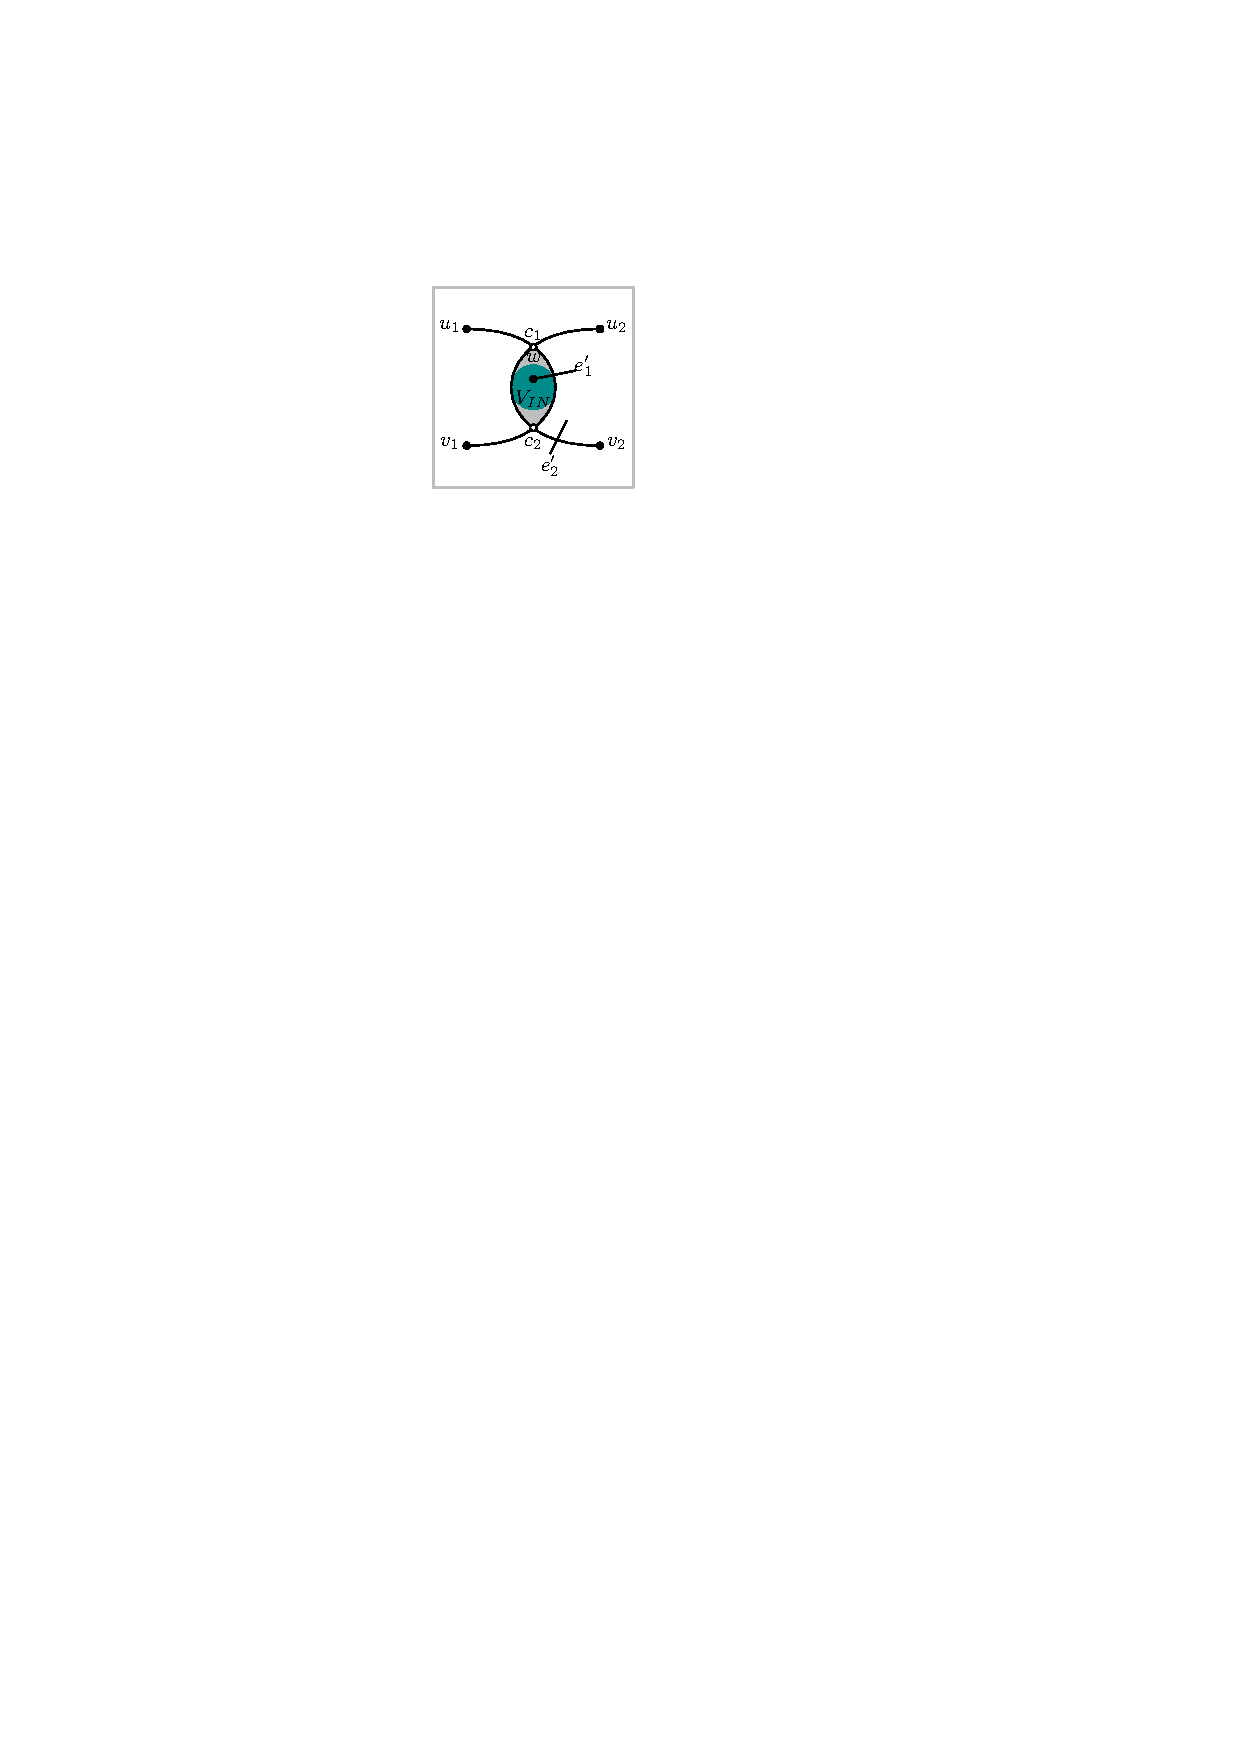
\includegraphics[width=\textwidth,page=1]{images/3_planar_cross_twice}
        \subcaption{~}\label{fig:3_planar_cross_twice_general}
    \end{minipage}
    \begin{minipage}[b]{.24\textwidth}
        \centering
        \includegraphics[width=\textwidth,page=2]{images/3_planar_cross_twice}
        \subcaption{~}\label{fig:3_planar_cross_twice_region}
    \end{minipage}
		\begin{minipage}[b]{.24\textwidth}
        \centering
        \includegraphics[width=\textwidth,page=3]{images/3_planar_cross_twice}
        \subcaption{~}\label{fig:3_planar_cross_twice_single}
    \end{minipage}
    \begin{minipage}[b]{.24\textwidth}
        \centering
        \includegraphics[width=\textwidth,page=4]{images/3_planar_cross_twice}
        \subcaption{~}\label{fig:3_planar_cross_twice_main}
    \end{minipage}
    \caption{%
    (a)-(d):~Configurations used in Lemma~\ref{lem:3_planar_cross_twice}.
    \label{fig:3_planar_one_crossing_2}}
\end{figure}

By combining Lemmas~\ref{lem:3_planar_faces_final} and \ref{lem:3_planar_cross_twice}, we can characterize all optimal $3$-planar graphs:


 By Lemma~\ref{lem:3_planar_cross_twice} we have that Lemma~\ref{lem:3_planar_faces_final} holds for all maximal $3$-planar graphs. Since the true planar subgraph of such a graph contains only faces of length $6$, we can start with a $6$-tiling of the plane\todo{rephrase}. Now in the interior of every face of length $6$, we can add all  $8$ missing edges using the $3$-planar pattern of Figure~\ref{fig:3_planar_polygon_conf_6}.
 %By Lemma~\ref{lem:3_planar_faces_final} we can characterize all maximal $3$-planar graphs. Since the true planar subgraph of such a graph contains only faces of length $6$, we can start with a $6$-tiling of the plane. Now in the interior of every face of length $6$, we can add all  $8$ missing edges.



% ============================================================================
\section{Conclusions}
\label{sec:conclusions}
% ============================================================================

In this paper, we developed techniques that allow us to characterize optimal $2$- and $3$-planar graphs. In particular, we had to deal with non-homotopic parallel edges, loops and also crossing adjacent edges, which required special attention and efforts. Natural extensions of our results would be to characterize optimal $4$-planar graphs, optimal fan-planar and quasi-planar graphs. But it would also be interesting to have a characterization of the simple versions of these graph classes where (non-homotopic) parallel edges and loops are forbidden. Another interesting line of research is the recognition of optimal $2$- and $3$-planar graphs. We note here the recent result by Brandenburg~\cite{DBLP:journals/corr/Brandenburg16a} who gives a linear time algorithm for the recognition of optimal $1$-planar graphs.

To Discuss:

\begin{itemize}
  \item Discussion on the desity of simple.
  \item Relation between optimal 2-planar and bar-1-visible.
  \item Relation between optimal 2-planar and 1-bend RAC.
\end{itemize}

% ============================================================================
\bibliographystyle{abbrv}
\bibliography{references}
% ============================================================================

\end{document}
